%%%%%%%%%%%%%%%%%%%%%%%%%%%%%%%%%%%%%%%%%%%%%%%%%%%%%%%%%%%%%%%%%%%%%%%%%%%%%%%%
%% Plantilla de memoria en LaTeX para la ETSIT - Universidad Rey Juan Carlos
%%
%% Por Gregorio Robles <grex arroba gsyc.urjc.es>
%%     Grupo de Sistemas y Comunicaciones
%%     Escuela Técnica Superior de Ingenieros de Telecomunicación
%%     Universidad Rey Juan Carlos
%% (muchas ideas tomadas de Internet, colegas del GSyC, antiguos alumnos...
%%  etc. Muchas gracias a todos)
%%
%% La última versión de esta plantilla está siempre disponible en:
%%     https://github.com/gregoriorobles/plantilla-memoria
%%
%% Para obtener PDF, ejecuta en la shell:
%%   make
%% (las imágenes deben ir en PNG o JPG)

%%%%%%%%%%%%%%%%%%%%%%%%%%%%%%%%%%%%%%%%%%%%%%%%%%%%%%%%%%%%%%%%%%%%%%%%%%%%%%%%

\documentclass[a4paper, 12pt]{report}
\usepackage[T1]{fontenc}

%                          DEBO ELIMINAR AL TERMINAR 
%%%%%%%%%%%%%%%%%%%%%%%%%%%%%%%%%%%%%%%%%%%%%%%%%%%%%%%%%%%%%%%%%%%%%%%%%%%%%%%%%
\usepackage{xcolor} %Definir colores
%%%%%%%%%%%%%%%%%%%%%%%%%%%%%%%%%%%%%%%%%%%%%%%%%%%%%%%%%%%%%%%%%%%%%%%%%%%%%%%%%
\usepackage{graphicx}
\usepackage{lscape}
\usepackage[a4paper, left=2.5cm, right=2.5cm, top=3cm, bottom=3cm]{geometry}
\usepackage{times}
\usepackage[spanish,es-tabla]{babel} % Comenta esta línea si tu memoria es en inglés
\spanishdecimal{.}
\usepackage{url}
%\usepackage[dvipdfm]{graphicx}

%make lists editable
%\usepackage{enumitem}
\usepackage{amsmath}
\usepackage{multirow} %tablas con multifila
\usepackage{graphicx}
\usepackage[utf8]{inputenc}
\usepackage[breaklinks=true]{hyperref} %% Para marcadores
\usepackage{float}  %% H para posicionar figuras
\usepackage[nottoc, notlot, notlof, notindex]{tocbibind} %% Opciones de índice
\usepackage{latexsym}  %% Logo LaTeX
\usepackage{csquotes}  %% Paquete para citas (displayquote)
\usepackage{amsthm}  %% Paquete para Teoremas
\usepackage{color}  %% Paquete para texto en color
\usepackage[normalem]{ulem}  %% Para tablas
\useunder{\uline}{\ul}{}  %% Para tablas
\usepackage{listings}  %% para código y comandos
\usepackage{pdfpages}  %% para incluir archivos PDF
\usepackage{enumerate}  %% Para enumerar
\usepackage[parfill]{parskip}  %% Párrafos
% Load the package

\usepackage[nice]{nicefrac} %nicefracview
\usepackage[nopostdot,style=super,nonumberlist,toc]{glossaries}
\usepackage[font=footnotesize,labelfont=bf]{caption}
\usepackage{subcaption}
% Generate the glossary
%Term definitions

%\setlength{\glsdescwidth}{5.5in}

%%%AUI HAY UN GRAVE PROBLEMA CON EL LINE BREAK

\makeglossaries
\newglossaryentry{wcg}{
    name={$\mathbf{WCG}$},
    description={\textit{Wide Color Gamut}}
}

\title{Memoria del Proyecto}
\author{Eduardo Durán Fuentes}

\renewcommand{\baselinestretch}{1.5}  %% Interlineado

\begin{document}

\renewcommand{\refname}{Bibliografía}  %% Renombrando
\renewcommand{\appendixname}{Apéndice}

%%%%%%%%%%%%%%%%%%%%%%%%%%%%%%%%%%%%%%%%%%%%%%%%%%%%%%%%%%%%%%%%%%%%%%%%%%%%%%%%
% PORTADA

\begin{titlepage}
\begin{center}
\begin{tabular}[c]{c c}

\includegraphics[scale=0.25]{img/0_portada/1_urjc_logo.png} &
\begin{tabular}[b]{l}
\Huge
\textsf{UNIVERSIDAD} \\
\Huge
\textsf{REY JUAN CARLOS} \\
\end{tabular}
\\
\end{tabular}

\vspace{3cm}

\Large
{INGENIERÍA EN SISTEMAS AUDIOVISUALES Y MULTIMEDIA}

\vspace{0.4cm}

\large
Curso Académico 2017/2018

\vspace{0.8cm}

Trabajo Fin de Grado

\vspace{2.5cm}

\Large
ANÁLISIS DE LA CONVERSIÓN DE CONTENIDOS HDR PARA LOS FORMATOS PQ Y HLG
\vspace{3cm}

\large
Autor : Eduardo Durán Fuentes \\
Tutor : Damián Ruiz Coll \\
Co-tutor : Miguel Ángel Santiago Cabello
\end{center}
\end{titlepage}

\newpage
\mbox{}
\thispagestyle{empty} % para que no se numere esta pagina


%%%%%%%%%%%%%%%%%%%%%%%%%%%%%%%%%%%%%%%%%%%%%%%%%%%%%%%%%%%%%%%%%%%%%%%%%%%%%%%%gls

%%%% Dedicatoria

\chapter*{}
\pagenumbering{Roman} % para comenzar la numeracion de paginas en numeros romanos
\begin{flushright}
\textit{Dedicado a \\
mi familia / mi abuelo / mi abuela}
\end{flushright}

%%%%%%%%%%%%%%%%%%%%%%%%%%%%%%%%%%%%%%%%%%%%%%%%%%%%%%%%%%%%%%%%%%%%%%%%%%%%%%%%
%%%% Agradecimientos

\chapter*{Agradecimientos}
%\addcontentsline{toc}{chapter}{Agradecimientos} % si queremos que aparezca en el índice
\markboth{AGRADECIMIENTOS}{AGRADECIMIENTOS} % encabezado 

Aquí vienen los agradecimientos\ldots Aunque está bien acordarse de la pareja, no hay que olvidarse de dar las gracias a tu madre, que aunque a veces no lo parezca disfrutará tanto de tus logros como tú\ldots 
Además, la pareja quizás no sea para siempre, pero tu madre sí.

%%%%%%%%%%%%%%%%%%%%%%%%%%%%%%%%%%%%%%%%%%%%%%%%%%%%%%%%%%%%%%%%%%%%%%%%%%%%%%%%
%%%% Resumen

\chapter*{Resumen}
%\addcontentsline{toc}{chapter}{Resumen} % si queremos que aparezca en el índice
\markboth{RESUMEN}{RESUMEN} % encabezado

Aquí viene un resumen del proyecto. Ha de constar de tres o cuatro párrafos, donde se presente de manera clara y concisa de qué va el proyecto. 
Han de quedar respondidas las siguientes preguntas:

\begin{itemize}
  \item De qué va este proyecto? Cuál es su objetivo principal?
  \item Cómo se ha realizado? Qué tecnologías están involucradas?
  \item En qué contexto se ha realizado el proyecto? Es un proyecto
dentro de un marco general?
\end{itemize}

Lo mejor es escribir el resumen al final.

%%%%%%%%%%%%%%%%%%%%%%%%%%%%%%%%%%%%%%%%%%%%%%%%%%%%%%%%%%%%%%%%%%%%%%%%%%%%%%%%
%%%% Resumen en inglés

\chapter*{Summary}
%\addcontentsline{toc}{chapter}{Summary} % si queremos que aparezca en el índice
\markboth{SUMMARY}{SUMMARY} % encabezado

Here comes a translation of the ``Resumen'' into English. Please, double check it for correct grammar and spelling.
As it is the translation of the ``Resumen'', which is supposed to be written at the end, this as well should be filled out
just before submitting.
%%%%%%%%%%%%%%%%%%%%%%%%%%%%%%%%%%%%%%%%%%%%%%%%%%%%%%%%%%%%%%%%%%%%%%%%%%%%%%%%
%%%% Glosario
\printglossaries
\glsaddall
\chapter*{Glosario}
\markboth{GLOSARIO}{GLOSARIO} % encabezado
\addcontentsline{toc}{chapter}{Glosario}
% Use the terms
\pagenumbering{arabic}
\newpage


%%%%%%%%%%%%%%%%%%%%%%%%%%%%%%%%%%%%%%%%%%%%%%%%%%%%%%%%%%%%%%%%%%%%%%%%%%%%%%%%
%%%%%%%%%%%%%%%%%%%%%%%%%%%%%%%%%%%%%%%%%%%%%%%%%%%%%%%%%%%%%%%%%%%%%%%%%%%%%%%%
% ÍNDICES %
%%%%%%%%%%%%%%%%%%%%%%%%%%%%%%%%%%%%%%%%%%%%%%%%%%%%%%%%%%%%%%%%%%%%%%%%%%%%%%%%

% Las buenas noticias es que los índices se generan automáticamente.
% Lo único que tienes que hacer es elegir  cuáles quieren que se generen,
% y comentar/descomentar esa instrucción de LaTeX.

%%%% Índice de contenidos
\tableofcontents 
%%%% Índice de figuras
\addcontentsline{toc}{chapter}{Índice de figuras} % para que aparezca en el indice de contenidos
\listoffigures % indice de figuras
%%%% Índice de tablas
%\cleardoublepage
%\addcontentsline{toc}{chapter}{Lista de tablas} % para que aparezca en el indice de contenidos
%\listoftables % Índice de tablas


%%%%%%%%%%%%%%%%%%%%%%%%%%%%%%%%%%%%%%%%%%%%%%%%%%%%%%%%%%%%%%%%%%%%%%%%%%%%%%%%
%%%%%%%%%%%%%%%%%%%%%%%%%%%%%%%%%%%%%%%%%%%%%%%%%%%%%%%%%%%%%%%%%%%%%%%%%%%%%%%%
% INTRODUCCIÓN %
%%%%%%%%%%%%%%%%%%%%%%%%%%%%%%%%%%%%%%%%%%%%%%%%%%%%%%%%%%%%%%%%%%%%%%%%%%%%%%%%

\cleardoublepage
\chapter{Introducción}
\label{sec:intro} % etiqueta para poder referenciar luego en el texto con ~\ref{sec:intro}

\section{Contexto}
\label{sec:seccion}
Desde hace años, los sensores de los dispositivos de captación con capaces de percibir rangos de color más  extensos que los que finalmente son representados en un dispositivo de visualización de consumidor. Este hecho puede observarse en la Figura \ref{fig:sdr_vs_hdr}.
\begin{figure}[H]
    \centering
    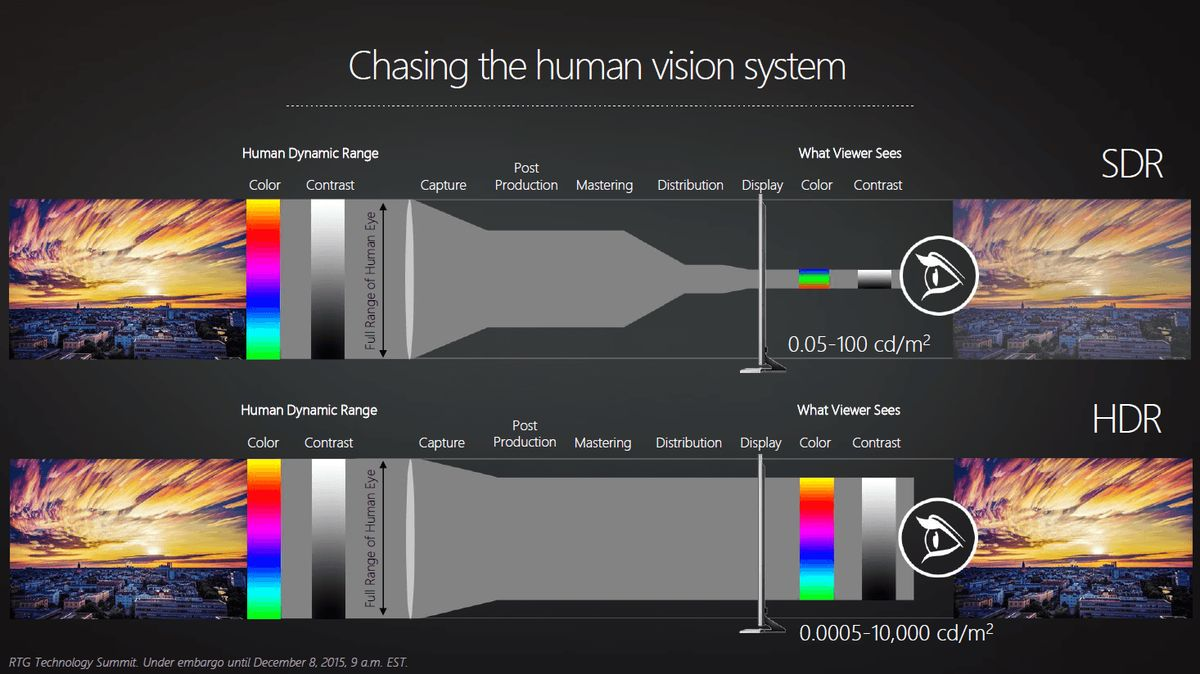
\includegraphics[width=14cm, keepaspectratio]{img/1_Introduccion/1_1_Contexto/1_hdr_sdr_range.jpg}
    \caption{Comparativa de los flujos de trabajo SDR y HDR. Credit: AMD RADEON RTG}
    \label{fig:sdr_vs_hdr}
\end{figure}
Con el objetivo de aprovechar las capacidades de estos sensores, surge la tecnología \textcolor{green}{wcg}, capaz de extender el rango de colores representables en las normativas anteriores.
La recomendación \textit{ITU-R BT.2020} se propone un espacio de color en el que  el cálculo de las cromaticities de los componentes primarios está directamente relacionado con las longitudes de onda puras de éstos. Es este el espacio de color utilizado por los sistemas de televisión \textcolor{green}{hdr}.

En la Figura \ref{fig:709_vs_2020} , se puede observar que el gamut de color \textit{ITU-R BT.2020} es mucho más amplio que el de la \textit{ITU-R BT.709}.

\begin{figure}[H]
    \centering
    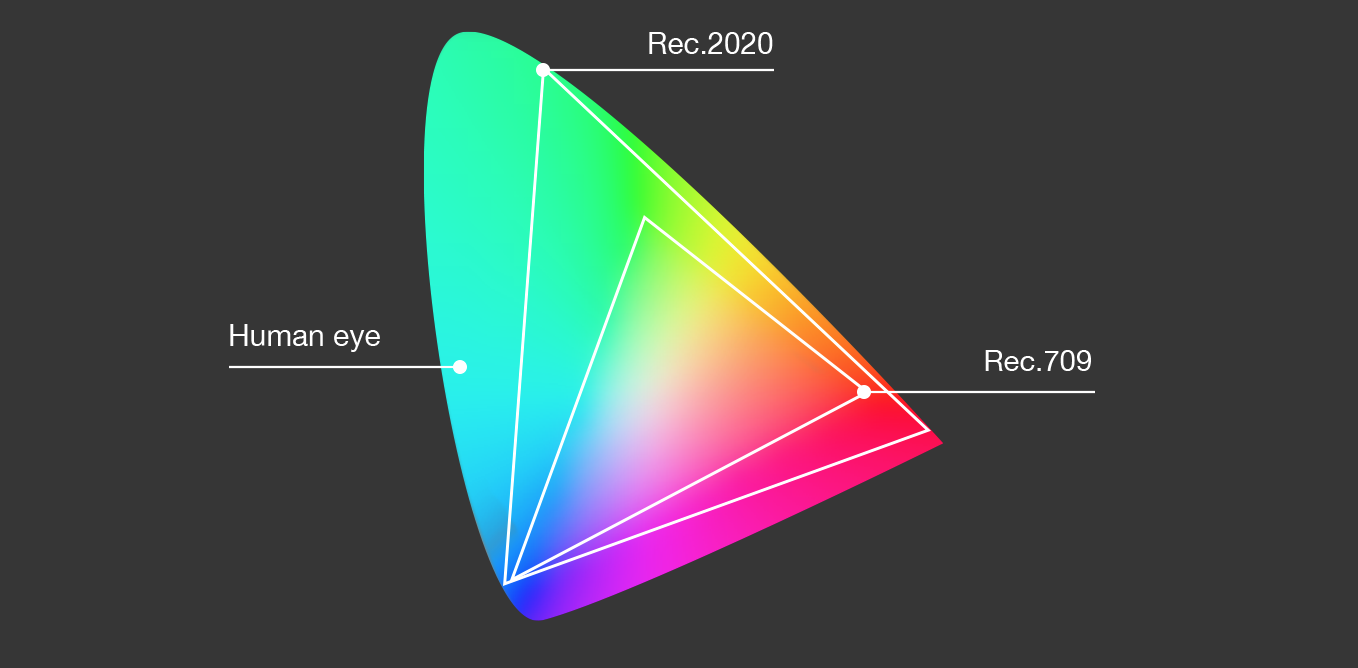
\includegraphics[width=12cm, keepaspectratio]{img/1_Introduccion/1_1_Contexto/2_709_vs_2020.png}
    \caption{Comparativa de los espacios de color \textit{ITU-R BT.709} y \textit{ITU-R BT.2020} Credit: tengo que buscarlo o poner otra imagen}
    \label{fig:709_vs_2020}
\end{figure}

\section{Motivación}
\label{sec:motivacion}


\section{Estructura del proyecto}
\label{sec:estructura}



%%%%%%%%%%%%%%%%%%%%%%%%%%%%%%%%%%%%%%%%%%%%%%%%%%%%%%%%%%%%%%%%%%%%%%%%%%%%%%%%
%%%%%%%%%%%%%%%%%%%%%%%%%%%%%%%%%%%%%%%%%%%%%%%%%%%%%%%%%%%%%%%%%%%%%%%%%%%%%%%%
% OBJETIVOS %
%%%%%%%%%%%%%%%%%%%%%%%%%%%%%%%%%%%%%%%%%%%%%%%%%%%%%%%%%%%%%%%%%%%%%%%%%%%%%%%%

\cleardoublepage % empezamos en página impar
\chapter{Objetivos} % título del capítulo (se muestra)
\label{chap:objetivos} % identificador del capítulo (no se muestra, es para poder referenciarlo)

\section{Objetivo general} % título de sección (se muestra)
\label{sec:objetivo-general} % identificador de sección (no se muestra, es para poder referenciarla)

\section{Objetivos específicos}
\label{sec:objetivos-especificos}

\section{Planificación temporal}
\label{sec:planificacion-temporal}


%%%%%%%%%%%%%%%%%%%%%%%%%%%%%%%%%%%%%%%%%%%%%%%%%%%%%%%%%%%%%%%%%%%%%%%%%%%%%%%%
%%%%%%%%%%%%%%%%%%%%%%%%%%%%%%%%%%%%%%%%%%%%%%%%%%%%%%%%%%%%%%%%%%%%%%%%%%%%%%%%
% FUNDAMENTOS DE TELEVISIÓN %
%%%%%%%%%%%%%%%%%%%%%%%%%%%%%%%%%%%%%%%%%%%%%%%%%%%%%%%%%%%%%%%%%%%%%%%%%%%%%%%%

\cleardoublepage
\chapter{Fundamentos de televisión}

\section{Formatos de televisión tradicionales}
\label{sec:formatos_tv}
La totalidad de los formatos de televisión, definición estándar o \textcolor{green}{sd}, alta definición o \textcolor{green}{hd} y ultra alta definición o \textcolor{green}{uhd}, están definidos por el \textit{ITU-R} en las siguientes recomendaciones:

\begin{itemize}
    \item \textbf{Definición estándar \textcolor{green}{sd}:} \textit{ITU-R BT.601}~\cite{itu_r:_bt601}.
    \item \textbf{Alta definición \textcolor{green}{hd}:} \textit{ITU-R BT.709}~\cite{itu_r:_bt709}.
    \item \textbf{Ultra alta definición \textcolor{green}{uhd}:} \textit{ITU-R BT.2020}~\cite{itu_r:_bt2020}.
\end{itemize}

Todos ellos tienen en común la definición de una serie de parámetros que los caracteriza, como son:

\begin{enumerate}[1]
    \item Colorimetría.
    \item Espacio de color.
    \item Resolución espacial y temporal.
    \item Profundidad de píxel.
    \item Submuetreo de croma.
\end{enumerate}

\subsection{Colorimetría}
\label{subsec:colorimetria_tv_trad}

El \textcolor{green}{hvs} es el sistema encargado de la captación, procesado e interpretación de imágenes. Se compone de dos órganos principales: el ojo y el cerebro, cuyas funciones son la captación e interpretación de imágenes, respectivamente.
El comportamiento de una cámara fotográfica es análogo al del ojo humano. De acuerdo con la imagen de la Figura \ref{fig:fotocamera}, determinadas funciones que desempeñan ciertos elementos de una cámara se corresponden con las que realizan algunas partes del ojo humano:


%\caption{Analogía entre el ojo humano y una cámara fotográfica\protect\footnotemark.}
\begin{itemize}
    \item  El iris del ojo humano se ajusta en función de intensidad lumínica de la escena, determinando la cantidad de luz que pasa al otro lado de éste a través de su centro: la pupila. De modo similar, el diafragma de una cámara fotográfica tiene como objetivo la regulación de la cantidad de luz de la escena que pasa al interior de ella.
    \item En el ojo humano, a través del ajuste de los músculos ciliares, el cristalino adopta la posición adecuada para lograr la composición óptima de la imagen en la retina. Ésta, a su vez, está formada por dos tipos de fotoreceptores:   
        \begin{enumerate}
            \item \textbf{Los conos: } se dividen en tres grupos de células, cuya excitación máxima ante la intensidad lumínica se produce a tres longitudes de onda diferentes del espectro visible: aproximadamente las correspondientes al rojo, verde y azul.
            Estas células son las encargadas de la visión cromática.
            \item \textbf{Los bastones: }tienen mayor sensibilidad lumínica que los conos. Por ello son las células encargadas de la visión nocturna o \textit{escotópica} y, por tanto, de la percepción de aspectos tales como el contorno de los objetos.
        \end{enumerate}
        De modo similar, por medio de un complejo sistema de lentes, en la cámara se ajusta el objetivo hasta conseguir el enfoque adecuado para lograr la correcta formación de la imagen en la película fotosensible o sensor digital, para cámaras analógicas o digitales, respectivamente.
\end{itemize}

\begin{figure}[H]
    \centering
    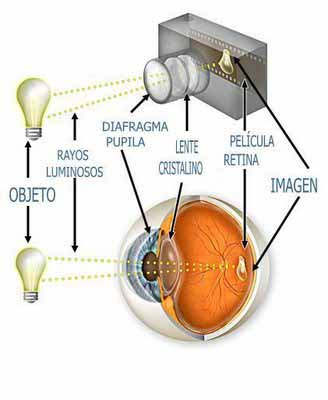
\includegraphics[width=6cm, keepaspectratio]{img/3_Fundamentos_de_Television/3_1_Formatos_de_TV_Tradicionales/3_1_1_Colorimetria/1_camera_vs_eye.jpg}
    \caption[Analogía entre el ojo humano y una cámara fotográfica]{Analogía entre el ojo humano y una cámara fotográfica~\cite{url:_ojo_camara}}
    \label{fig:fotocamera}
\end{figure}

Teniendo en cuenta la respuesta del ojo humano ante diferentes longitudes de onda, en 1931, la organización \textcolor{green}{cie}\textcolor{red}{~\cite{nondefined:_cie1931}}(El CIE-15 lo reemplaza(2004))  desarrolló un diagrama  en el cual se representan el conjunto de colores que es capaz de percibir el ojo humano. El diseño de este sistema, designado como \textit{CIE XYZ 1931}\textcolor{red}{(Añadir enlace bibliográfico)}, se basó en las funciones \textit{colour matching} definidas para un observador estándar, las cuales se representan en la Figura \ref{fig:tristimulus_cie2d} (a).

En este sistema, las coordenadas \textit{XYZ}, conocidas como \textit{tristimulus} son obtenidas como la proyección de la distribución espectral de intensidad luminosa sobre las funciones $\overline{x}$, $\overline{y}$ y $\overline{z}$. En la fase de diseño del sistema,  se decidió  que \textit{XYZ} pudieran tomar sólo valores positivos, siendo \textit{Y} proporcional a la luminancia de la mezcla aditiva de las tres componentes, mientras que \textit{X} y \textit{Z} contienen información colorimética. En el diagrama tridimensional  de la Figura \ref{fig:tristimulus_cie2d} \textbf{(b)}, la diagonal se corresponde con la zona acromática, es decir, los niveles de grises, donde $X=Y=Z$.\

\begin{figure}[H]
    \centering
    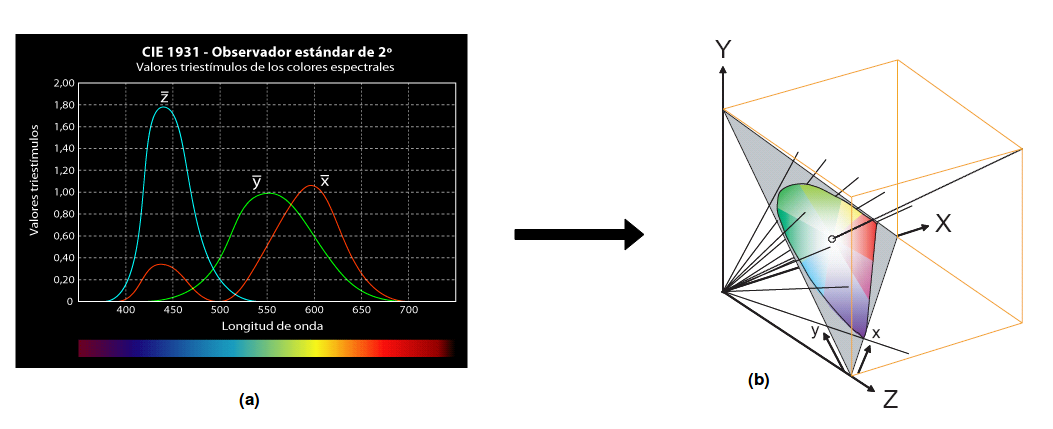
\includegraphics[width=14cm, keepaspectratio]{img/3_Fundamentos_de_Television/3_1_Formatos_de_TV_Tradicionales/3_1_1_Colorimetria/2_tristimulus_cie3d.png}
    \caption{(a) Funciones \textit{colour matching} observador estándar, (b) Diagrama \textit{CIE 1931 XYZ}}
    \label{fig:tristimulus_cie2d}
\end{figure}
%\begin{figure}[H]
%\begin{subfigure}{.5\textwidth}
%  \centering
%  \includegraphics[width=.8\linewidth]{img/triestimulus.png}
%  \caption{a}
%  \label{fig:sfig1}
%\end{subfigure}%
%\begin{subfigure}{.5\textwidth}
%  \centering
%  \includegraphics[width=.8\linewidth]{img/3dcie1931.png}
%  \caption{b}
%  \label{fig:sfig2}
%\end{subfigure}
%\caption{plots of....}
%\label{fig:fig}
%\end{figure}

 Se definen tres coordenadas (\textit{x}, \textit{y}, \textit{z}), obtenidas a partir de los \textit{tristimulus XYZ}, según la Ecuación \ref{eq:xyz_coords}.
\footnotesize
\begin{equation}
    \begin{aligned}
        x = \frac{X}{X + Y + Z}\qquad y = \frac{Y}{X + Y  + Z}&\qquad z = \frac{Z}{X + Y + Z} \\
        x + y + z = 1 &
    \end{aligned}
    \label{eq:xyz_coords}
\end{equation}
\normalsize

 A fin de obtener una representación del color sin tener en cuenta la luminancia, el \textcolor{green}{cie} propone un diagrama bidimensional, conocido como \textit{CIE xy}. Este diagrama, mostrado en la Figura \ref{fig:CIExy1931}, se define por convenio en el plano \textit{xy}. Dentro de esta superficie están contenidas todas las posibles combinaciones colorimétricas visibles por el ojo humano, en cuanto a saturación y tono se refiere. Sin embargo, está desacoplado de la luminancia.
 
 Para poder observar las variaciones de luminancia para cada combinación tono-saturación es necesario obtener la componente \textit{z} asociadada a cada par \textit{(x, y)}. De este modo se puede construir un volumen formado por la combinación planos \textit{xy}, donde la componente \textit{z} puede ser extraída a través de la siguiente igualdad: $x + y + z = 1$.
 
 \begin{figure}[H]
    \centering
    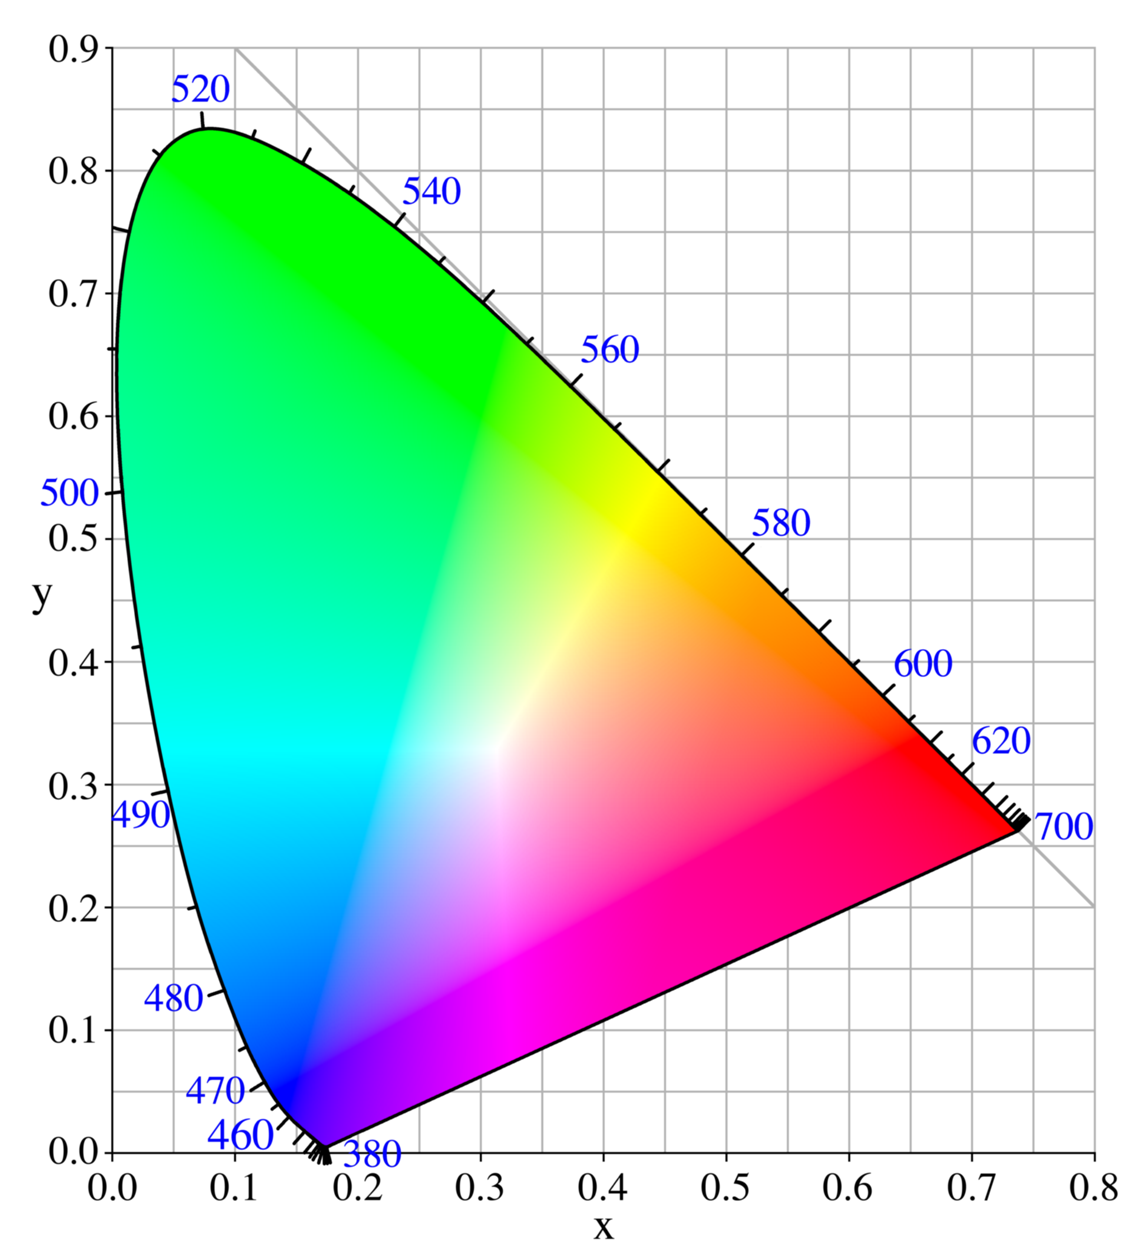
\includegraphics[width=9cm, keepaspectratio]{img/3_Fundamentos_de_Television/3_1_Formatos_de_TV_Tradicionales/3_1_1_Colorimetria/3_CIExy1931.png}
    \caption{Diagrama \textit{CIE 1931 XYZ}}
    \label{fig:CIExy1931}
\end{figure}

\subsection{Espacio de color: RGB, YCbCr}
\label{subsec:colorspace}
Un espacio de color es una representación matemática que define un conjunto de colores idealmente representables en un monitor. Éste se define por las coordenadas (\textit{x,y}) de sus componentes primarias y las del blanco de referencia en el \textit{CIE 1931 XYZ}.


Existen diferentes espacios de color, de los cuales, en televisión son utilizados los siguientes:
\begin{itemize}
    \item \textbf{RGB:} El espacio de color RGB es un sistema no perceptual basado en el modelo de color aditivo\footnote{El modelo de color RGB es aditivo, es decir, en él  un determinado color es generado mediante la combinación de luces correspondientes a diferentes longitudes de onda. Se consideran como colores primarios las luces cuya longitud de onda se corresponde con el rojo (\textit{Red}), verde (\textit{Green}) y azul (\textit{Blue}), que dan nombre  a dicho modelo.} con el mismo nombre. Tal y como se puede observar en la Figura \ref{fig:rgbcube}, se utiliza un sistema cartesiano en tres dimensiones para representar el conjunto de todos los colores definidos por éste.
\end{itemize}
%puedes hacer combinaciones de estas cosas hasta lograr la apariencia deseada%
\begin{figure}[H]
    \centering
    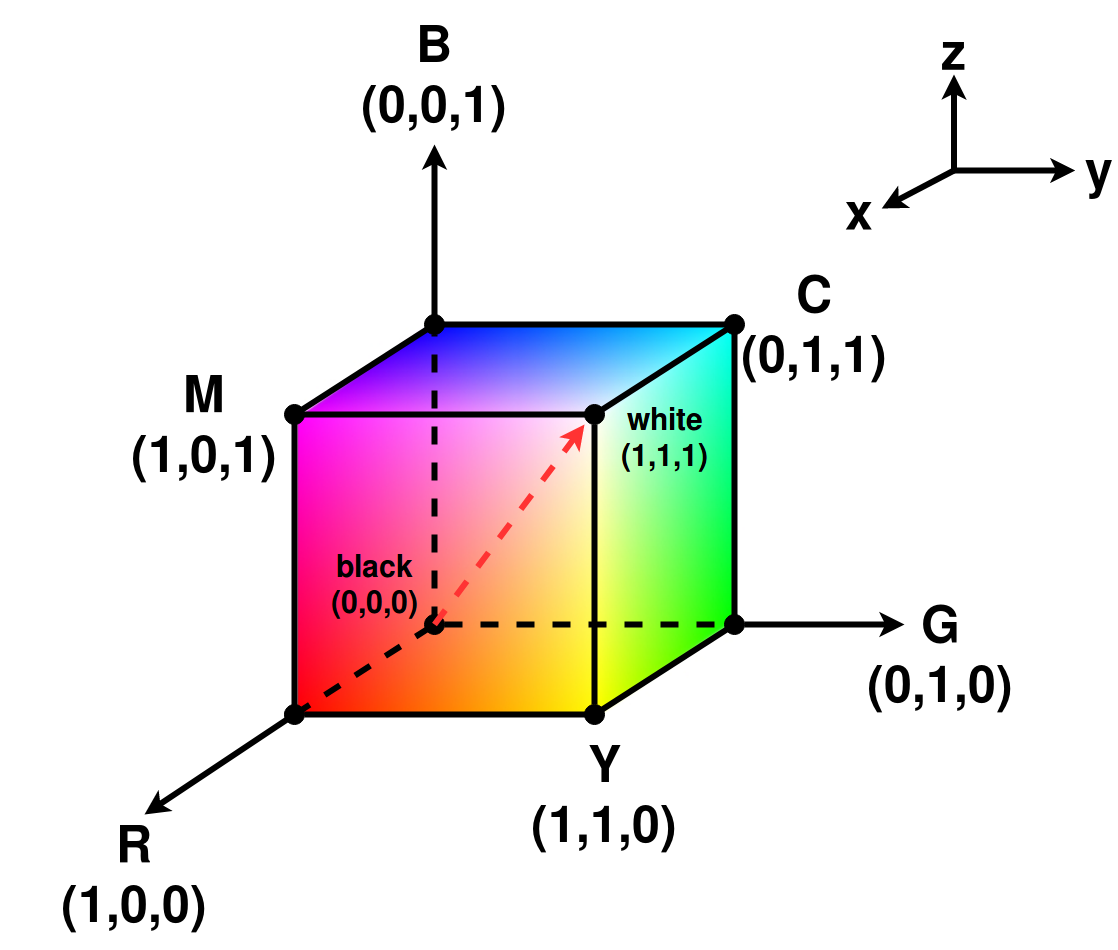
\includegraphics[width=14cm, height=9cm]{img/3_Fundamentos_de_Television/3_1_Formatos_de_TV_Tradicionales/3_1_2_Espacios_de_Color/1_rgb_cube.png}
    \caption{Representación cartesiana del espacio de color RGB}
    \label{fig:rgbcube}
\end{figure}

\begin{itemize}
    \item Los colores primarios (RGB) son representados en los vértices (1,0,0), (0,1,0) y (0,0,1), respectivamente.
    \item El resto de colores se producen como resultado de la combinación de los anteriores. De este modo, los vértices (1,1,0), (1,0,1) y (0,1,1)
     se correspenden con los colores amarillo, \textit{cyan} y magenta, respectivamente.
     \item La diagonal representa los colores acromáticos, es decir, aquellos colores compuestos por la misma aportación de cada una de las componentes primarias RGB, siendo el origen de coordenadas (0,0,0) la ausencia de intensidad lumínica (negro), y el vértice (1,1,1), el punto de máxima intensidad (blanco). El resto de colores contenidos en la diagonal acromática se corresponden con la escala de grises.
\end{itemize}
 Este espacio de color es utilizado por los sensores de las cámaras y  en los sistemas de televisión. Sin embargo, existen diferencias en función del formato y la resolución. En Europa ha sido estandarizado por el EBU (ITU-R BT.470), tanto para televisión digital como analógica.

%Como el espacio de color RGB es no perceptual, no tiene en cuenta la respuesta no lineal del ojo humano ante diferentes longitudes de onda del espectro visible, es decir, no considera que la sensibilidad de las células fotorreceptoras de éste no es constante con la longitud de onda.%

Para mapear cualquier porcentaje del cubo \textcolor{green}{rgb} (especificado por cada sistema de televisión) a un sistema perceptual, como el CIE 1931 XY, deben seguirse las indicaciones de la recomendación RP-177~\cite{smpte:_rp177}, desarrolladas en el Anexo \ref{sec:rgb_to_xyz}.
 

 
 %En los sistemas de televisión, (tal y como se ha mencionado anteriormente), el modo en que la energía luminosa de la escena es traducida a las señales eléctricas que representan las componentes \textcolor{green}{rgb} no es lineal con el modo en que un monitor traduce estas componentes del dominio eléctrico al óptico. Por tanto, las componentes \textcolor{green}{rgb} de entrada ($R_S, G_S, B_S$) al sistema tienen valores diferentes que las de salida ($R_D, G_D, B_D$). %

Debido a razones de compatibilidad entre dispositivos de visualización, puede ser necesaria la conversión entre los diferentes gamuts de color definidos por los sistemas de televisión \textcolor{green}{sd},\textcolor{green}{sd} \textcolor{green}{hd} y \textcolor{green}{uhd}. Para ello, la recomendación RP-177~\cite{smpte:_rp177} especifica el método explicado en el Anexo \ref{sec:rgbs_to_rgbd}, el cuál también es válido para la transformación de coordenadas \textcolor{green}{rgb} de referencia a coordenadas \textcolor{green}{rgb} de visualización.

En la Tabla. \ref{TABLE:COL_TV} se concretan las coordenadas que definen el \textcolor{green}{gamut} de los sistemas de televisión.

\begin{table}[H]
\resizebox{\textwidth}{!}{%
\begin{tabular}{|c|c|c|c|l|l|}
\hline
\multicolumn{2}{|c|}{\multirow{2}{*}{\textbf{Sistema de TV}}}                                                                        & \multicolumn{2}{c|}{ITU-R BT.601 (SD)}                                                                                                & \multirow{2}{*}{ITU-R BT.709 (HD)} & \multirow{2}{*}{ITU-R BT.2020 (UHD)} \\ \cline{3-4}
\multicolumn{2}{|c|}{}                                                                                                               & \begin{tabular}[c]{@{}c@{}}NTSC \\ (Sistema americano)\end{tabular} & \begin{tabular}[c]{@{}c@{}}PAL\\ (Sistema europeo)\end{tabular} &                                    &                                      \\ \hline
\multirow{3}{*}{\textbf{\begin{tabular}[c]{@{}c@{}}Coordenadas de \\ cromaticidad (x,y)\\ en el CIE 1931\end{tabular}}} & \textbf{R} & (0.630,0.340)                                                       & (0.640,0.330)                                                   & (0.640,0.330)                      & (0.708,0.292)                        \\ \cline{2-6} 
                                                                                                                        & \textbf{G} & (0.310,0.595)                                                       & (0.290,0.600)                                                   & (0.300,0.600)                      & (0.170,0.797)                        \\ \cline{2-6} 
                                                                                                                        & \textbf{B} & (0.155,0.070)                                                       & (0.150,0.060)                                                   & (0.150,0.060)                      & (0.131,0.046)                        \\ \hline
\multicolumn{2}{|c|}{\textbf{\begin{tabular}[c]{@{}c@{}}Coordenadas del\\ blanco de referencia\\ (D65) en el CIE 1931\end{tabular}}} & \multicolumn{4}{c|}{(0.3127,0.3290)}                                                                                                                                                                              \\ \hline
\end{tabular}%
}
\caption{Coordenadas \textit{(x,y)} en los sistemas de televisión SD, HD y UHD.}
\label{TABLE:COL_TV}
\end{table}

Tal y como se desarrolla en la Sección \ref{subsec:croma_sub}, el ojo humano es más sensible a las variaciones de luminosidad que a las de tono y saturación del color. Este hecho permite que en los sistemas de televisión sea posible ahorrar ancho de banda por medio de la reducción de la información de color sin que sea percibido de modo subjetivo por un observador. Para poder realizar esta tarea es necesario separar la información de luma de la de croma. El espacio de color YCbCr cubre esta necesidad.

\begin{itemize}
    \item \textbf{YCbCr:} Es una espacio de color que permite separar completamente la información de luma de la de croma. En él, una imagen se define por tres componentes:  una de luma (Y) y dos de diferencia de color (Cb, Cr), siendo Cb la representación de las escala tonal entre y azul y el amarillo; y Cr la ubicación de los colores entre el rojo y el verde.
\end{itemize}
En el documento de prácticas recomendadadas RP-177~\cite{smpte:_rp177} se describen las ecuaciones que permiten derivar las componentes ($Y$, $C_{b}$, $C_{r}$) a partir de las coordenadas ($x,y,z$) de las componentes \textcolor{green}{rgb} de un determinado \textcolor{green}{gamut} de color.

En los sistemas de televisión tradicionales (\textcolor{green}{sdr}), se utilizan espacios de color cuyas coordenadas \textit{xy} de las componentes primarias fueron calculadas basándose en las emisiones luminosas de los fósforos de los monitores \textcolor{green}{crt}: los espacios de color de \textcolor{green}{sd} y \textcolor{green}{hd}.

Mediante la representación de las coordenadas anteriores en el diagrama \textcolor{green}{cie} , se obtienen las superficies triangulares mostradas en la Figura  \ref{fig:cie_diagram}, que representan el \textit{gamut} de color de los sistemas de televisión. Tal y como se puede observar en \textbf{(a)}, los rangos colorimétricos de \textcolor{green}{sd} y \textcolor{green}{hd} son muy similares. En cambio, de acuerdo con \textbf{(b)}, el rango de colores  de \textcolor{green}{uhd} es mucho más extenso que el de los dos sistemas de televisión anteriores, lo que posibilita representar colores más saturados , es decir, más \textit{vivos}.



\begin{figure}[H]
    \centering
    
\includegraphics[width=14cm, keepaspectratio]{img/no_image.jpg}
    \caption{ Representación de los espacios de color SD, HD y UHD en el diagrama CIE 1931 xy.}
    \label{fig:cie_diagram}
\end{figure} 

\subsection{Profundidad de píxel}
\label{subsec:color_depth}

\begin{table}[H]
\centering
\resizebox{\textwidth}{!}{%
\begin{tabular}{|c|c|c|c|c|}
\hline
\multirow{2}{*}{\textbf{Sistema de TV}}                                                    & \multicolumn{2}{c|}{ITU-R BT.601 (SD)}                                                                                                & \multirow{2}{*}{ITU-R BT.709 (HD)} & \multirow{2}{*}{ITU-R BT.2020 (UHD)} \\ \cline{2-3}
                                                                                           & \begin{tabular}[c]{@{}c@{}}NTSC \\ (Formato americano)\end{tabular} & \begin{tabular}[c]{@{}c@{}}PAL\\ (Formato europeo)\end{tabular} &                                    &                                      \\ \hline
\textbf{\begin{tabular}[c]{@{}c@{}}Profundidad\\ de píxel\\ {[}bits/píxel{]}\end{tabular}} & \multicolumn{2}{c|}{8, 10}                                                                                                            & 8, 10                              & 10, 12                               \\ \hline
\end{tabular}%
}
\caption{Profundidad de píxel en los sistemas de televisión SD, HD y UHD}
\label{table:bit_depth}
\end{table}


\subsection{Submuestreo de croma}
\label{subsec:croma_sub}

El ojo humano tiene menor sensibilidad a las variaciones cromáticas (tono y saturación) que a las luminosas. Debido a este hecho, en los contenidos audiovisuales existe información relativa al color que no va ser percibida por el ojo humano, la cual se conoce como \textit{redundancia subjetiva}.
Si estos contenidos son transformados de \textcolor{green}{rgb} a $YC_{b}C_{r}$, la información cromática se encuentra aislada de la lumínica. En este formato de imagen es posible eliminar la \textit{redundancia subjetiva} por medio del submuestreo de croma. En los sistemas de televisión existen los siguientes formatos:
\begin{itemize}
    \item \textbf{4:4:4.} Mismo número de componentes (\textit{Y'},\textit{Cb'}, \textit{Cr'}).
    \item \textbf{4:2:2.} Se toman la mitad de las muestras de las componentes  de croma (\textit{Cb'}, \textit{Cr'}), en sentido  horizontal, con respecto a las muestras de luma(\textit{Y'}).
    \item \textbf{4:2:0.} Se toman la mitad de las muestras de las componentes  de croma (\textit{Cb'}, \textit{Cr'}), tanto en sentido  horizontal como vertical, con respecto a las muestras de luma(\textit{Y'}).
\end{itemize}
En la Figura \ref{fig:chroma_sub} se indican los formatos de submuestreo de croma soportados por cada uno de los sistemas de televisión.
\begin{figure}[H]
    \centering
    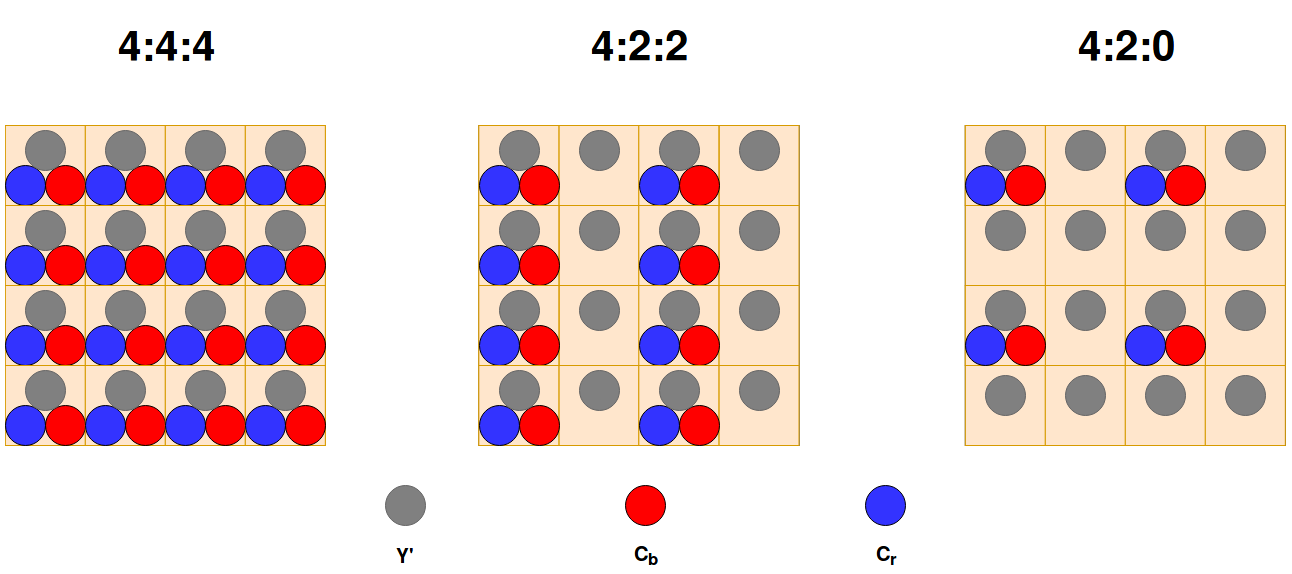
\includegraphics[width=9cm, keepaspectratio]{img/3_Fundamentos_de_Television/3_1_Formatos_de_TV_Tradicionales/3_1_4_Submuestreo_de_Croma/1_chroma_subsampling.png}
    \caption{Formatos de croma definidos en la recomendación ITU-R BT.2100}
    \label{fig:chroma_sub}
\end{figure}
\begin{table}[H]
\centering
\resizebox{\textwidth}{!}{%
\begin{tabular}{|c|c|c|c|c|}
\hline
\multirow{2}{*}{\textbf{Sistema de TV}}                                                       & \multicolumn{2}{c|}{ITU-R BT.601 (SD)} & \multirow{2}{*}{ITU-R BT.709 (HD)} & \multirow{2}{*}{ITU-R BT.2020 (UHD)} \\ \cline{2-3}
                                                                                              & NTSC               & PAL               &                                    &                                      \\ \hline
\textbf{\begin{tabular}[c]{@{}c@{}}Submuestreo de\\  las componentes\\ de croma\end{tabular}} & \multicolumn{3}{c|}{4:4:4, 4:2:2}                                           & 4:4:4, 4:2:2, 4:2:0                  \\ \hline
\end{tabular}%
}
\caption{Submuestreo de croma en los sistemas de televisión SD, HD y UHD.}
\label{table:croma_sub}
\end{table}

\subsection{Resolución espacial y temporal}
\label{subsec:res_esp_temp}

\begin{table}[H]
\centering
\resizebox{\textwidth}{!}{%
\begin{tabular}{|c|l|l|l|l|}
\hline
\multirow{2}{*}{\textbf{Sistema de TV}}                                                      & \multicolumn{2}{l|}{ITU-R BT.601 (SD)}                                                                                                              & \multirow{2}{*}{ITU-R BT.709 (HD)}                                                                                                                                                                                                                                                                                                                                                                                          & \multirow{2}{*}{ITU-R BT.2020 (UHD)}                                                                                                                                                                                                                                            \\ \cline{2-3}
                                                                                             & NTSC                                                                           & PAL                                                                &                                                                                                                                                                                                                                                                                                                                                                                                                             &                                                                                                                                                                                                                                                                                 \\ \hline
\textbf{\begin{tabular}[c]{@{}c@{}}Resolución \\ \\ espacial\\ (píxeles/frame)\end{tabular}} & 720x 480                                                                       & 720x576                                                            & \begin{tabular}[c]{@{}l@{}}1260x720 \\ 1920x1080\end{tabular}                                                                                                                                                                                                                                                                                                                                                               & \begin{tabular}[c]{@{}l@{}}UHD-1: 3840x2160\\ UHD-2: 7680x4320\end{tabular}                                                                                                                                                                                                     \\ \hline
\textbf{Resolución temporal (Hz)}                                                            & \begin{tabular}[c]{@{}l@{}}Entrelazado:\\ 60/1.001i (30/1.001 Hz)\end{tabular} & \begin{tabular}[c]{@{}l@{}}Entrelazado:\\ 50i (25 Hz)\end{tabular} & \begin{tabular}[c]{@{}l@{}}Progresivo: \\ \\ 24p (24 Hz), 25p (25 Hz), 30p (30 Hz),\\ 50p (50 Hz),60p (60 Hz).\\ \\ 24/1.001p (24/1.001 Hz), 30/ 1.001p (30/1.001 Hz),\\  60/1.001p (60/1.001 Hz).\\ \\ Entrelazado:\\ 50i (25 Hz), 60i (30 Hz), 60/1.001i (30/1.001 Hz).\\ Frame segmentado: \\ \\ \\ 24 PsF (24 Hz), 25 PsF (25 Hz), 30 PsF (30 Hz),\\  24/1.001PsF (24/1.001 Hz) 30/1.001PsF (30/1.001 Hz).\end{tabular} & \begin{tabular}[c]{@{}l@{}}Progresivo: \\ \\ \\ 24p (24 Hz), 25p (25 Hz), 30p (30 Hz),\\  50p (50 Hz), 60p (60 Hz), 100p (100 Hz), \\ \\ 120p (120 Hz), 24/1.001p (24/1.001 Hz),\\  30/1.001p (30/1.001 Hz), 60/1.001p (60/1.001 Hz),\\  120/1.001p (120/1.001 Hz)\end{tabular} \\ \hline
\end{tabular}%
}
\caption{Resolución temporal y espacial en los sistemas de televisión SD, HD y UHD.}
\label{table:res}
\end{table}


\subsection{Función de transferencia}
\label{subsec:sistema_tv}
En un sistema de televisión, ya sea \textcolor{green}{sdr} o \textcolor{green}{hdr},  se distinguen tres funciones de transferencia, cuyo objetivo es la transformación de la señal de vídeo entre los dominios óptico y eléctrico.

\begin{itemize}
  \item  \textcolor{green}{oetf}: Es la función de transferencia óptico-eléctrica. Desempeña la función de mapear la luz lineal captada por la cámara de una determinada escena a una señal eléctrica, típicamente no lineal, que será enviada a través de los sistemas de distribución. Esta función se aplica comúmente en el interior de los dispositivos de captación.
  \item \textcolor{green}{eotf}: Es la función de transferencia eléctrico-óptica, que realiza el mapeo de la señal eléctrica no lineal a la intensidad lumínica de cada uno de los píxeles presentados por el dispositivo de visualización.
  
  Inicialmente surgió como la no linealidad existente entre la señal eléctrica transmitida a los tradicionales monitores \textcolor{green}{crt}, conocida como \textcolor{green}{gamma}, con un valor de $\gamma = 2.4$. La función de transferencia opto-eléctrica de la cámaras fue ajustada para compensar esta alinealidad.
  Sin embargo, por razones de conservación del contraste el resultado esperado de dicha corrección no debe ser totalmente lineal, sino una curva con un valor de $\gamma = 1.1$. Estas curvas se muestran en la Figura (\textcolor{red}{he representado estas funciones con la herramienta y me ha surgido una duda al compararlas con las diapositivas de Equipos. Lo comentamos en la reunión})
\end{itemize}
En un sistema de televisión, la intensidad luminosa que un dispositivo de captación es capaz de detectar  no es proporcional a la que un dispositivo de visualización puede presentar.

\begin{itemize}
  \item  \textcolor{green}{ootf}:  Es la función de transferencia opto-óptica. También designada como \textit{OOTF de referencia} o  \textit{función del sistema}, es la encargada de traducir la luz lineal de la escena capturada por la cámara en la luz presentada por pantalla.
    Esta función puede ser modificada a juicio de los profesionales del mástering y el etalonaje, a fin de conseguir el look deseado en la imagen, en función del género y estilo de contenido. En el caso de aplicarse estos ajustes, recibe el nombre de \textit{OOTF artística}.

\end{itemize}

Todas estas funciones de transferencia están relacionadas, de modo que una de ellas puede obtenerse a partir de las otras dos, a través de las expresiones definidas en la recomendación ITU-R BT.2390-4\footnote{\url{https://www.itu.int/pub/R-REP-BT.2390}}:\\
\footnotesize
\begin{subequations}
    \label{subeq:tf_def}
    \begin{eqnarray}
        &OETF_x(R, G, B) = EOTF^{-1}_x(OOTF_x(R, G, B)) \\ 
        &OETF^{-1}_x(R, G, B) = OOTF^{-1}_x(EOTF_x (R, G, B)) \\ 
        &EOTF_x(R, G, B) = OOTF_x(OETF^{-1}_x (R, G, B))  \\ 
        &EOTF^{-1}_x(R, G, B) = OETF_x(OOTF^{-1}_x (R, G, B)) \\            
        &OOTF_x(R, G, B) = EOTF_x(OETF_x (R, G, B)) \\
        &OOTF^{-1}_x(R, G, B) = OETF^{-1}_x(EOTF^{-1}_x (R, G, B))
    \end{eqnarray}
\end{subequations}
\normalsize
donde el  subíndice \textit{x} hace referencia a la  componente \textcolor{green}{rgb} sobre la que se aplica la transformación correspondiente.

%%%%%%%%%%%%%%%%%%%%%%%%%%%%%%%%%%%%%%%%%%%%%%%%%%%%%%%%%%%%%%%%%%%%%%%%%%%%%%%%
%%%%%%%%%%%%%%%%%%%%%%%%%%%%%%%%%%%%%%%%%%%%%%%%%%%%%%%%%%%%%%%%%%%%%%%%%%%%%%%%
% FORMATOS DE TELEVISIÓN DE ALTO RANGO DINÁMICO: ITU-R BT.2100 %
%%%%%%%%%%%%%%%%%%%%%%%%%%%%%%%%%%%%%%%%%%%%%%%%%%%%%%%%%%%%%%%%%%%%%%%%%%%%%%%%

\cleardoublepage
\chapter{Formatos de televisión de Alto Rango Dinámico: \textit{ITU-T BT.2100}}
\label{chap:formatos_hdr}


\section{Sistema PQ}
\label{sec:sistema_pq_teoria}

De acuerdo con la recomendación \textit{ITU-R BT.2100}~\cite{itu_r:_bt2100}, el sistema \textcolor{green}{pq} es referido al dispositivo de visualización. En consecuencia, su \textcolor{green}{eotf} se define de forma explícita. La Figura \ref{fig:pq_sist}, representa las tranformaciones sufridas por la señal de vídeo \textcolor{green}{pq} desde su captura hasta su visualización, las cuales son descritas en la Tabla \ref{table:pq_params}.

La \textcolor{green}{oetf}, en cambio, es derivada a través de la aplicación en cascada de \textcolor{green}{ootf} y \textcolor{green}{inveotf}.   
Las ecuaciones \ref{eq:eotf_pq}, \ref{eq:ootf_pq} y \ref{eq:inv_eotf_pq} permiten obtener la \textcolor{green}{eotf}, la \textcolor{green}{ootf} y la \textcolor{green}{inveotf}, respectivamente. En las figuras \ref{fig:pq_graph_oetf}, \ref{fig:pq_graph_eotf} y \ref{fig:pq_graph_ootf}  se representan la \textcolor{green}{oetf}, \textcolor{green}{eotf} y \textcolor{green}{ootf}, respectivamente.
\begin{figure}[H]
  \centering
  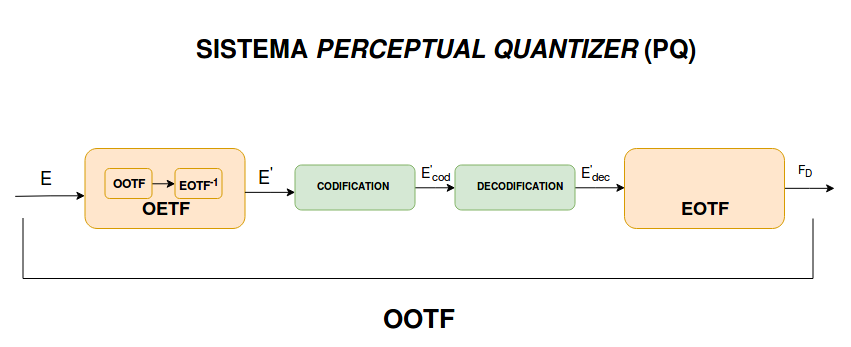
\includegraphics[width=12cm, keepaspectratio]{img/4_Formatos_de_TV_HDR/4_1_Sistema_PQ/1_Sistema_PQ.png}
  \caption{SISTEMA PQ}
  \label{fig:pq_sist}
\end{figure}

\begin{table}[H]
    \begin{tabular}{|p{1.25cm}| p{3cm}|p{10.5cm}| }
       \hline 
        \textbf{Señal} &\textbf{Rango} & \textbf{Descripción} \\ \hline
        $E$ &[$0,1$]  &  Señal obtenida a través de la luz de la escena, y escalada a través de la exposición de la cámara: \{$R_{s}$,$G_{s}$,$B_{s}$\}   \\\hline
        $E^{'}$ &[$0,1$]  & Señal no lineal aplicada sobre cada componente : \{$R^{'}$,$G^{'}$,$B^{'}$\} \\\hline
        $E^{'}_{cod}$&  No &  \textcolor{red}{Aqui tengo pensado explicar narrow range}\\\hline
        $E^{'}_{decod}$ &    & \\\hline
        $F_D$& [$0,10000$] $\nicefrac{cd}{m^{2}}$ & Luminancia de una componente lineal: \{$R_{D}$,$G_{D}$,$B_{D}$\} \\\hline
    \end{tabular}
    \caption{Señal PQ en diferentes puntos del sistema}
    \label{table:pq_params}
\end{table}

\footnotesize
\begin{equation} \label{eq:eotf_pq}
    F_D = EOTF[E^{'}] = 10000Y \\
    {\small \textrm{  , donde  }}\\ 
    Y= \left ( \frac{max[(E'^{\nicefrac{1}{m_2}} - c_1),0]}{c_2 -c_3E'^{\nicefrac{1}{m_2}}} \right)^{\nicefrac{1}{m_1}}
\end{equation}

\normalsize
\begin{itemize}
    \item {\small El parámetro $Y$ es definido como un color linear normalizado, en el rango $[0, 1]$. Se obtiene a través de la igualdad: {\footnotesize $$Y=\nicefrac{F_D}{10000}$$}}
    {\small \item $m_1$, $m_2$, $c_1$, $c_2$ y $c_3$  son constantes correspondientes a la fase de diseño del sistema \textcolor{green}{pq}, definidas en la recomendación \textit{ITU-R BT.2100}.}
\end{itemize}

\footnotesize
\begin{equation} \label{eq:oetf_pq}
    E^{'} = OETF[E] = EOTF^{-1}[OOTF[E]] = EOTF^{-1}[F_D]
\end{equation}

\begin{equation}  \label{eq:ootf_pq}
   F_D = OOTF[E] = 100E^{'^{2.4}} \textrm{  , donde  }\\
       E^{'}=% 
        \begin{cases}
            267.84E, & 0\leq E \leq 0.0003024\\
            1.099(59.5208E)^{0.45} - 0.099, &0.0003024 < E < 1
        \end{cases}
\end{equation}

\begin{equation} \label{eq:inv_eotf_pq}
    EOTF^{-1}[F_D] = \left ( \frac{c_1 + c_2Y^{m_1}}{1 + c_3Y^{m_1}} \right)^{m_2}\\
\end{equation}

\normalsize
\begin{figure}[H]
  \centering
  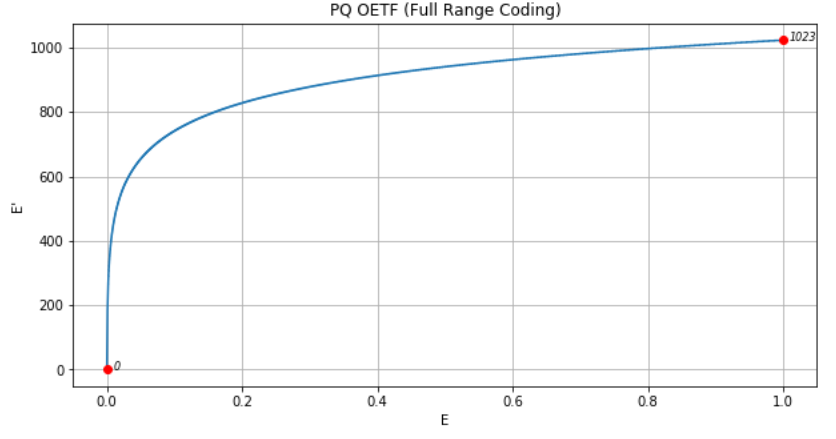
\includegraphics[width=12cm, keepaspectratio]{img/4_Formatos_de_TV_HDR/4_1_Sistema_PQ/2_oetf_full_range_log_lin.png}
  \caption{OETF PQ}
  \label{fig:pq_graph_oetf}
\end{figure}

\begin{figure}[H]
  \centering
  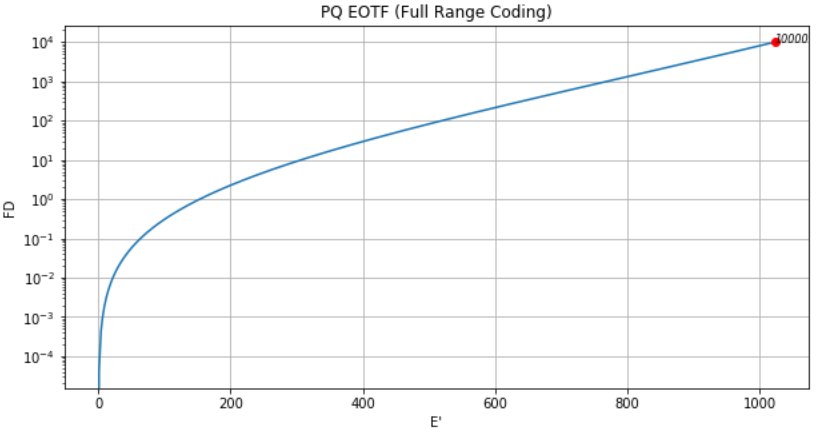
\includegraphics[width=12cm, keepaspectratio]{img/4_Formatos_de_TV_HDR/4_1_Sistema_PQ/3_eotf_full_range_log_lin.png}
  \caption{EOTF PQ}
  \label{fig:pq_graph_eotf}
\end{figure}

\textcolor{red}{(La OOTF tiene errores para niveles mínimos. Me gustaría revisar esto juntos)}
\begin{figure}[H]
  \centering
  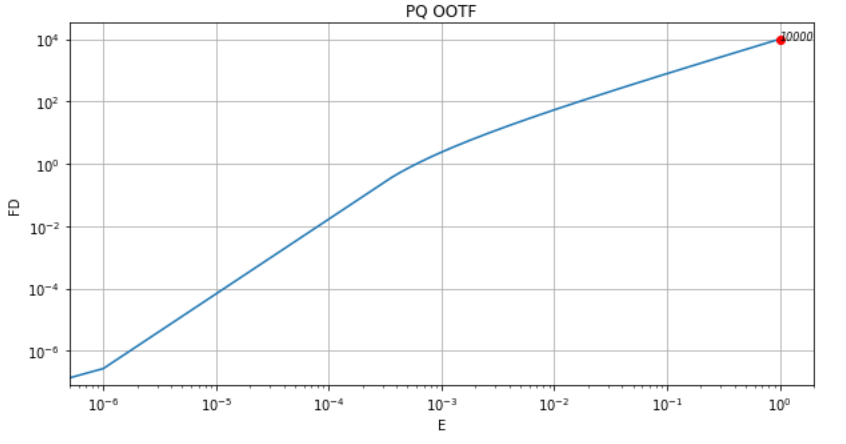
\includegraphics[width=12cm, keepaspectratio]{img/4_Formatos_de_TV_HDR/4_1_Sistema_PQ/4_ootf_log_log.png}
  \caption{OOTF PQ}
  \label{fig:pq_graph_ootf}
\end{figure}

\section{Sistema HLG}
\label{sec:sistema_hlg_teoria}

De acuerdo con la recomendación \textit{ITU-R BT.2100-1}, el sistema \textcolor{green}{hlg} es referido al dispositivo de captación. En consecuencia, es su \textcolor{green}{oetf} la función que se define de forma explícita. La Figura \ref{fig:hlg_sist} representa las tranformaciones sufridas por la señal de vídeo \textcolor{green}{hlg} desde su captura hasta su visualización, las cuales son descritas en la Tabla \ref{table:hlg_params}. 

Por otro lado, la \textcolor{green}{eotf} es derivada a través de la aplicación en cascada de \textcolor{green}{invoetf} y \textcolor{green}{ootf}.   
Las Ecuaciones \ref{eq:oetf_hlg}, \ref{eq:inv_oetf_hlg} y \ref{subeq:ootf_hlg} permiten obtener la \textcolor{green}{oetf}, la \textcolor{green}{invoetf} y la \textcolor{green}{ootf}, respectivamente. En las Figuras \ref{fig:hlg_graph_oetf}, \ref{fig:hlg_graph_eotf} y \ref{fig:hlg_graph_ootf}  se representan la \textcolor{green}{oetf}, \textcolor{green}{eotf} y \textcolor{green}{ootf}, respectivamente.
\begin{figure}[H]
  \centering
  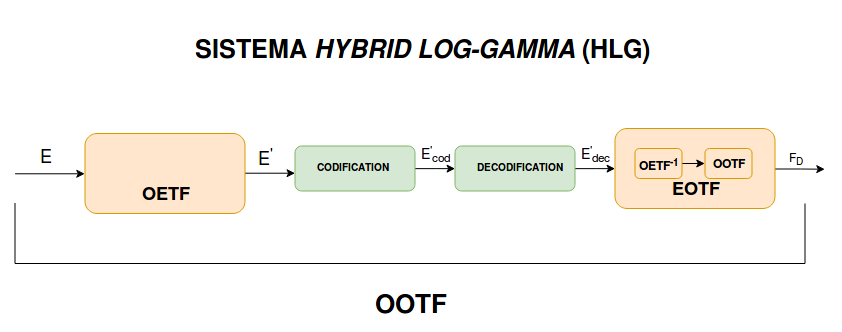
\includegraphics[width=12cm, keepaspectratio]{img/4_Formatos_de_TV_HDR/4_2_Sistema_HLG/1_Sistema_HLG.png}
  \caption{SISTEMA HLG}
  \label{fig:hlg_sist}
\end{figure}

\begin{table}[H]
    \begin{tabular}{|p{1.25cm}| p{3cm}|p{10.5cm}| }
       \hline 
        \textbf{Señal} &\textbf{Rango} & \textbf{Descripción} \\ \hline
        $E$ &[$0,1$]  &  Señal obtenida a través de la luz de la escena, y escalada a través de la exposición de la cámara: \{$R_{s}$,$G_{s}$,$B_{s}$\}   \\\hline
        $E^{'}$ &[$0,1$]  & Señal no lineal aplicada sobre cada componente : \{$R^{'}$,$G^{'}$,$B^{'}$\} \\\hline
        $E^{'}_{cod}$&    &  \\\hline
        $E^{'}_{decod}$ &    & \\\hline
        $F_D$& [$L_{B},L_{W}$] $\nicefrac{cd}{m^{2}}$ & Luminancia de una componente lineal: \{$R_{D}$,$G_{D}$,$B_{D}$\}, donde $L_B$  y $L_W$ son los niveles de luminancia mínimo y máximo del monitor objetivo, respectivamente. \\\hline
    \end{tabular}
    \caption{Señal HLG a través del sistema}
    \label{table:hlg_params}
\end{table}

\footnotesize
\begin{equation} \label{eq:oetf_hlg}
    E^{'}=OETF[E]% 
    \begin{cases}
        \sqrt{3E}, & 0\leq E \leq \nicefrac{1}{12}\\
        a\ln({12E - b}) +c, &\nicefrac{1}{12} < E < 1
    \end{cases}\qquad \textrm{,donde:}
\end{equation}
\normalsize
\begin{itemize}
    \item {\small El parámetro $Y$ es definido como un color linear normalizado, en el rango $[0, 1]$. Se obtiene a través de la igualdad: {\footnotesize $$Y=\nicefrac{F_D}{10000}$$}}
    {\small \item $a$, $b$  y $c$  son constantes correspondientes a la fase de diseño del sistema \textcolor{green}{hlg}, definidas en la recomendación \textit{ITU-R BT.2100}.}
\end{itemize}

\footnotesize
\begin{equation} \label{eq:eotf_hlg}
    F_D = EOTF[E] = OOTF[OETF^{-1}[E^{'}]] \textrm{  , donde  }\\
\end{equation}

\begin{equation}\label{eq:inv_oetf_hlg}
    E =OETF^{-1}[E^{'}]=% 
    \begin{cases}
        \nicefrac{E^{'^{2}}}{3}, & 0\leq E^{'} \leq \nicefrac{1}{2}\\
        \nicefrac{[exp(\nicefrac{(E^{'}- c)}{a}) + b]}{12}, & \nicefrac{1}{2} < E^{'} < 1
    \end{cases}
\end{equation}

\begin{subequations}
    \label{subeq:ootf_hlg}
    \begin{eqnarray}
        &F_D = OOTF[E] = \alpha Y_{s}^{\gamma -1}E + \beta & \\ 
        &R_D = OOTF[E] = \alpha R_{s}^{\gamma -1}E + \beta & \nonumber\\ 
        &G_D = OOTF[E] = \alpha G_{s}^{\gamma -1}E + \beta & \nonumber\\ 
        &B_D = OOTF[E] = \alpha B_{s}^{\gamma -1}E + \beta & \nonumber {\small \textrm{  , donde:}}\\
        \nonumber
    \end{eqnarray}
\end{subequations}

\begin{itemize}
     \item Los parámetros {\small $\alpha$ y $\beta$ se corresponden con el rango dinámico y el mínimo nivel lumínico del monitor objetivo ($L_B$), respectivamente. Las expresiones que los definen son las siguientes:{\footnotesize $$\alpha = L_w -L_B,\qquad \beta=L_B$$}}
     
      \item {\small El parámetro $\gamma$ se corresponde con la \textit{gamma} del sistema, que toma un valor de $\gamma=1.2$ para monitores con un nivel de luminancia pico $L_W=1000\, \nicefrac{cd}{m^{2}}$. Tal y como se puede observar en la siguiente ecuación,
      para valores superiores de $L_W$, el valor de la \textit{gamma} del sistema se incrementará.{\footnotesize $$\gamma=1.2 + 0.42Log_{10}(\nicefrac{L_W}{1000})$$}}
    \item {\small El parámetro $Y_s$ es la luminancia de la escena normalizada, y se define a través de : {\footnotesize $$Y_s= 0.2627R_s + 0.6780G_s + 0.0593B_s$$}}
\end{itemize}
\normalsize

\begin{figure}[H]
  \centering
  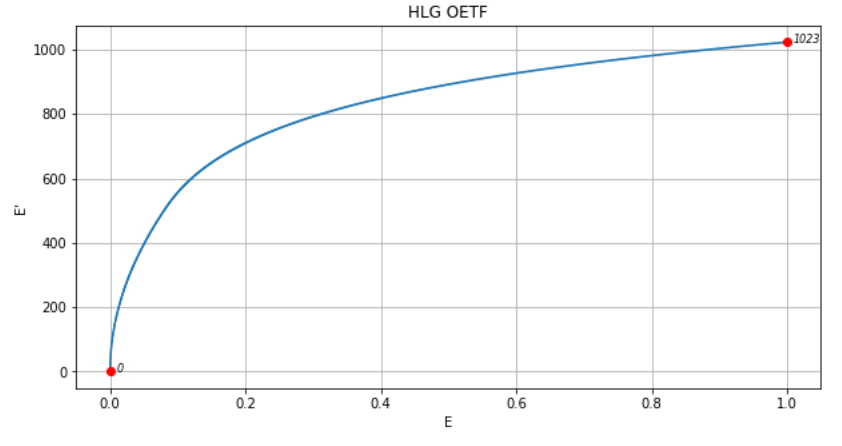
\includegraphics[width=12cm, keepaspectratio]{img/4_Formatos_de_TV_HDR/4_2_Sistema_HLG/2_oetf_lin_lin.png}
  \caption{OETF HLG}
  \label{fig:hlg_graph_oetf}
\end{figure}

\begin{figure}[H]
  \centering
  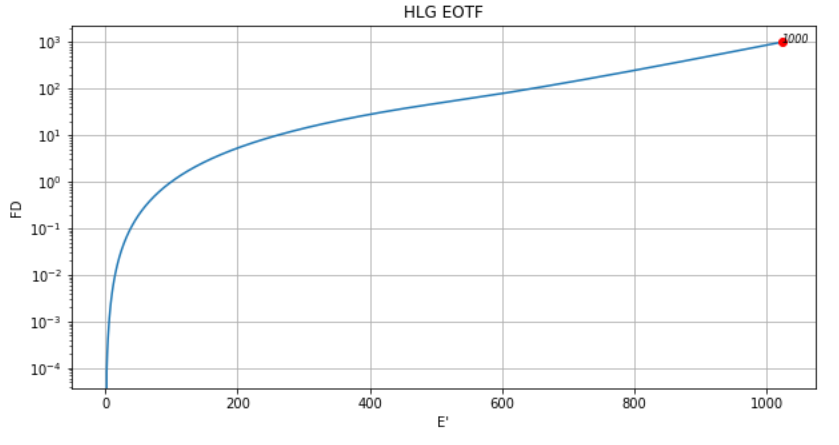
\includegraphics[width=12cm, keepaspectratio]{img/4_Formatos_de_TV_HDR/4_2_Sistema_HLG/3_eotf_log_lin.png}
  \caption{EOTF HLG}
  \label{fig:hlg_graph_eotf}
\end{figure}

\textcolor{red}{(La OOTF tiene errores para niveles mínimos. Me gustaría revisar esto juntos)}
\begin{figure}[H]
  \centering
  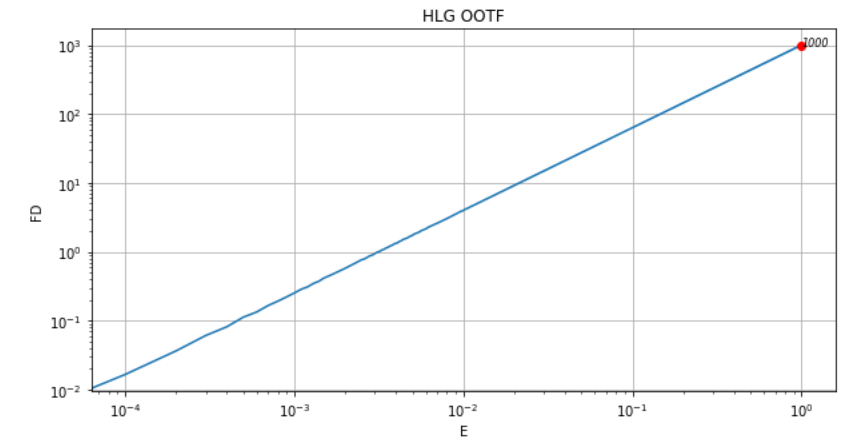
\includegraphics[width=12cm, keepaspectratio]{img/4_Formatos_de_TV_HDR/4_2_Sistema_HLG/4_ootf_log_log.png}
  \caption{OOTF HLG}
  \label{fig:hlg_graph_ootf}
\end{figure}

\section{Formatos de luminancia}
\label{sec:formatos_luminancia}
 El formato  de luminancia no constante (\textcolor{green}{ncl}) es el mecanismo que ha sido utilizado en los sistemas de televisión tradicionales para separar la componentes de croma de la luma.



La luma \textit{Y'} se obtiene por medio de la Ecuación \ref{eq:luma_ncl}, mientras que las componentes de diferencia de color, \textit{Cb’} y \textit{Cr’}, son obtenidas a través de la Ecuación \ref{eq:croma_ncl}.


\begin{equation} \label{eq:luma_ncl}
    Y^{'} = k_RR^{'} + k_GG^{'} + k_BB^{'}
\end{equation}

\begin{equation} \label{eq:croma_ncl}
    C_B^{'} = \frac{B^{'} - Y^{'}}{2(1 - k_B)} \qquad C_R^{'} = \frac{R^{'} - Y^{'}}{2(1 - k_R)}\\
\end{equation}

donde $k_R$, $k_G$ y $k_B$ son los coeficientes de ponderación de las componentes primarias, dependientes del espacio de color. En el caso de la \textit{ITU-R BT.2020}: $k_R = 0.2627$, $k_G = 0.6780$ y $k_B = 0.0593$.

Tal y como se describe en la recomendación \textit{ITU-R BT.2390}~\cite{itu_r:_bt2390}, las conversiones anteriores producen una serie de errores, que no eran perceptibles en los sistemas de televisión \textcolor{green}{sdr} tradicionales. 

Sin embargo, con el aumento de la extensión rangos colorimétricos y lumínicos ofrecidos por las tecnologías \textcolor{green}{wcg} y \textcolor{green}{hdr}, respectivamente, surgen los siguientes problemas:

\begin{itemize}
  \item Debido al aumento del volumen de color, las exigencias en profundidad de bit se incrementan, pudiendo producirse        distorsiones de cuantización al utilizar un número de bits por componente demasiado bajo.
  \item Pueden producirse incorrecciones en el mapeo  del volumen de color, debido a errores de cálculo en la predicción        del tono y la luminacia.
  \item En el caso del sistema \textcolor{green}{pq}, pueden producirse distorsiones en el submuestreo de croma, debidas la distribución no uniforme de las palabras de código tras aplicarse transformaciones perceptuales sobre las componentes \textcolor{green}{rgb}.
  \item Es posible observar propagación de errores de los canales de croma al de luma.
\end{itemize}

  En la recomendación \textit{ITU-R BT.2020} se propone un nuevo método de conversión, la conversión de luminancia constante (\textcolor{green}{cl}), que corrige la propagación de errores entre canales de croma y luma. Sin embargo, no ha sido adoptado por la recomendación \textit{ITU-R BT.2100}, ya que el coste en complejidad es demasiado alto para la gravedad del problema que  enmienda.
  
  \textcolor{red}{Queda pendiente decidir si añado ICtCp o no}


\section{Agudeza visual}
\label{sec:agudeza_visual}
 
 En los sistemas de televisión tradicionales o \textcolor{green}{sdr}, las funciones \textcolor{green}{eotf} no se definen de forma explícita
en sus respectivas recomendaciones: \textit{ITU-R BT.601} y \textit{ITU-R BT.709}. Esto se debe a que, tal y como se decribe en \textit{ITU-R BT.1886}~\cite{itu_r:_bt1886}, en aquella época tanto los monitores utilizados en producción como en visualización eran  \textcolor{green}{crt}, es decir, con características similares. Sin embargo, cada fabricante de televisores implementaba su propia \textcolor{green}{eotf} en función del modelo y región, pudiendo variar sus características de acuerdo a la modificación  de los ajustes de brillo y contraste por parte del consumidor. 
Con la llegada de los monitores de pantalla plana, se incrementó el uso de este tipo de dispositivos, de características diferentes a los \textcolor{green}{crt}, en entornos de producción. Debido a este cambio y a la diversidad de \textcolor{green}{eotf}s existentes en el mercado, la recomendación \textit{ITU-R BT.1886} propuso una función de transferencia electro-óptica de referencia común a todos los monitores utilizados en la produción de contenidos \textcolor{green}{hd}, a fin de grantizar la consisitencia de estos. Esta función se define en la Ecuación \ref{eq:bt_1886_1}.

\footnotesize
\begin{equation} \label{eq:bt_1886_1}
    L= a (max[(V + b),0])^{\gamma},\textrm{  donde:}
\end{equation}
\begin{itemize}
    \item $L$ es la luminancia del monitor objetivo.
    \item  $\gamma$, con un valor de $2'4$, es el exponente responsable de la adaptación a las pantallas \textcolor{green}{crt}.
    \item  $V  \in (0, 1)$ es la señal de vídeo normalizada, donde los valores 0 y 1 se corresponden con los colores acromáticos negro y blanco, respectivamente.
    \item $a$ y $b$ son los parámetros de control de contraste y brillo regulables por el usuario, respectivamente. Ambos parámetros son dependientes de $\gamma$ y de los niveles de luminancia mínimo ($L_{b}$) y máximo ($L_{w}$) de la pantalla objetivo.
\end{itemize}

\normalsize
En determinadas pantallas planas puede ocurrir que la función anterior no sea lo suficientemente precisa como para adaptar los contenidos producidos a una pantalla \textcolor{green}{crt} sin perder el \textit{look} original. En esta situación debe utilizarse una mejor aproximación, definida en la Ecuación \ref{eq:bt_1886_2}.

\footnotesize
\begin{equation} \label{eq:bt_1886_2}
    L=% 
    \begin{cases}
        k (V + b)^{\alpha_{2}} (V_{c} + b)^{\alpha_{1} - \alpha_{2}}, &  V < V_{c}\\
        k (V + b)^{\alpha_{1}} , &  V \geq V_{c}\qquad\textrm{, donde:}
    \end{cases}
\end{equation}

\begin{itemize}
    \item $L$, $\gamma$, $V$ y $b$ se definen en la Ecuación \ref{eq:bt_1886_1}.
    \item  $V_{c}=0.35$, $\alpha_{1}=2.6$, $\alpha_{2}=3.0$ y $k$ es un coeficiente de normalización.
\end{itemize}

\normalsize
De acuerdo con \textit{Perceptual Signal Coding for More Efficient Usage of Bit Codes}~\cite{smpte:_barten}, el modelo de Barten~\cite{csf:_barten_1,csf:_barten_2} proporciona una buena aproximación  de la función \textcolor{green}{csf}, la cual representa la sensibilidad al contraste del ojo humano. Este modelo está basado en mediciones empíricas de carácter físico y óptico; y en resultados obtenidos a través de experimentos y tests de carácter subjetivo. \textcolor{red}{Puedo extenderme en hablar sobre los JNDs, pero creo que se va a quedar muy largo.}.

Este modelo permite definir un umbral por debajo del cual el ojo humano no es capaz de percibir \textit{artefactos} derivados de errores de cuantificación, tales como el efecto  de \textit{banding} o zonas planas. Este efecto será más notable cuanto menor número de palabras de código se utilicen para representar el rango de niveles de luminancia que un monitor es capaz de producir. Existe, por tanto , una dependencia de la profundidad de bit en la definición del umbral de Barten. Éste relaciona el paso de contraste con el rango de niveles de luminancia que un monitor es capaz de representar. 


En las Figuras \ref{fig:barten_10} y \ref{fig:barten_12}  se muestra la relación \textit{paso de contraste-rango dinámico} de las \textcolor{green}{eotf}\textbf{s} de \textcolor{green}{pq}, el sistema \textcolor{green}{hd} (\textit{ITU-R BT.1886}) y el umbral de Barten, con precisiones de 10 y 12 bits, respectivamente.

En estas figuras se observa que:
\begin{itemize}
    \item El umbral de Barten, tanto para 10 como 12 bits, es menor en niveles de luminancia altos que en bajos. Esto quiere decir que el ojo humano tiene mayor sensibilidad al contraste en altas luces que en bajas. Sin embargo, a partir de un cierto porcentaje del paso de contraste se observa una zona de saturación a partir de la cual, con independencia del nivel de luminancia el ojo humano no es capaz de percibir \textit{banding} en la imagen. Esto ocurre aproximadamente por debajo del 0,7\%  y 0.5\% de paso de contraste para 12 y 10 bits, respectivamente.
    
    \item Por otro lado, la relación \textit{paso de contraste-rango dinámico} es lineal para la \textcolor{green}{eotf}  de la \textit{ITU-R BT.1886}, tanto para niveles pico de 100 $\nicefrac{cd}{m^{2}}$ como para 10000 $\nicefrac{cd}{m^{2}}$. Esto significa que, al no ajustarse a la tendencia del umbral de Barten, la \textit{gamma} utilizada para la definición de esta curva no se acomoda a la respuesta del ojo humano al contraste. En consecuencia:
    \begin{enumerate}
        \item En los sistemas \textcolor{green}{sdr}, con un nivel de luminancia pico  de 100 $\nicefrac{cd}{m^{2}}$, esta recta queda totalmente bajo el umbral de Barten, si  se utilizan 12 bits en la codificación. Sin embargo, si se reduce la profundidad de bit a 10 bits, se observa que en el rango 0.01-10 $\nicefrac{cd}{m^{2}}$, dicha recto se sitúa sobre el umbral, En dicho rango, se percibirán efectos de\textit{banding}.
        \item Si se utiliza la misma curva para  \textcolor{green}{hdr}, con un nivel de luminancia pico de 10000 $\nicefrac{cd}{m^{2}}$, se observa que esta función se sitúa sobre el umbral de Barten en los rangos 0.001-2000 y 0.001-80 $\nicefrac{cd}{m^{2}}$ para 10 y 12 bits, respectivamente. En este caso, la cantidad de \textit{artefactos} de cuantización percibidos por el ojo humano es muy elevada.
    \end{enumerate}
\end{itemize}

En conclusión, la falta de precisión de la \textit{ITU-R BT.1886} para ajustarse al \textcolor{green}{hvs} hace que esta curva sea ineficiente, ya que asigna un número de palabras de código demasiado pequeño para niveles de luminancia bajos y desperdicia en niveles altos, ya que no tiene en cuenta la zona de saturación presente en ambas figuras.

Para sistemas de televisión \textcolor{green}{hdr} es necesario, por tanto, el diseño de una nueva \textcolor{green}{eotf} que represente con fidelidad la respuesta al contraste del ojo humano: la curva \textcolor{green}{pq}, cuya relación \textit{paso de contraste-rango dinámico} se basa en las mismas ecuaciones utilizadas para la definición del umbral de Barten. En el caso de 12 bits, dicha curva se encuentra totalmente por debajo del umbral. Sin embargo, en contraposición a \textit{ITU-R BT.1886}, no desperdicia palabras de código.

Por otro lado, en el caso de 10 bits, toda la curva se encuentra sobre el umbral, lo que teóricamente significa que se produce el efecto de \textit{banding}. Sin embargo, en un sistema de televisión real, los niveles de ruido enmascaran este efecto para los casos de \textcolor{green}{pq} a 10000 $\nicefrac{cd}{m^{2}}$ e \textit{ITU-R BT.1886} a 100 $\nicefrac{cd}{m^{2}}$

\begin{figure}[H]
  \centering
  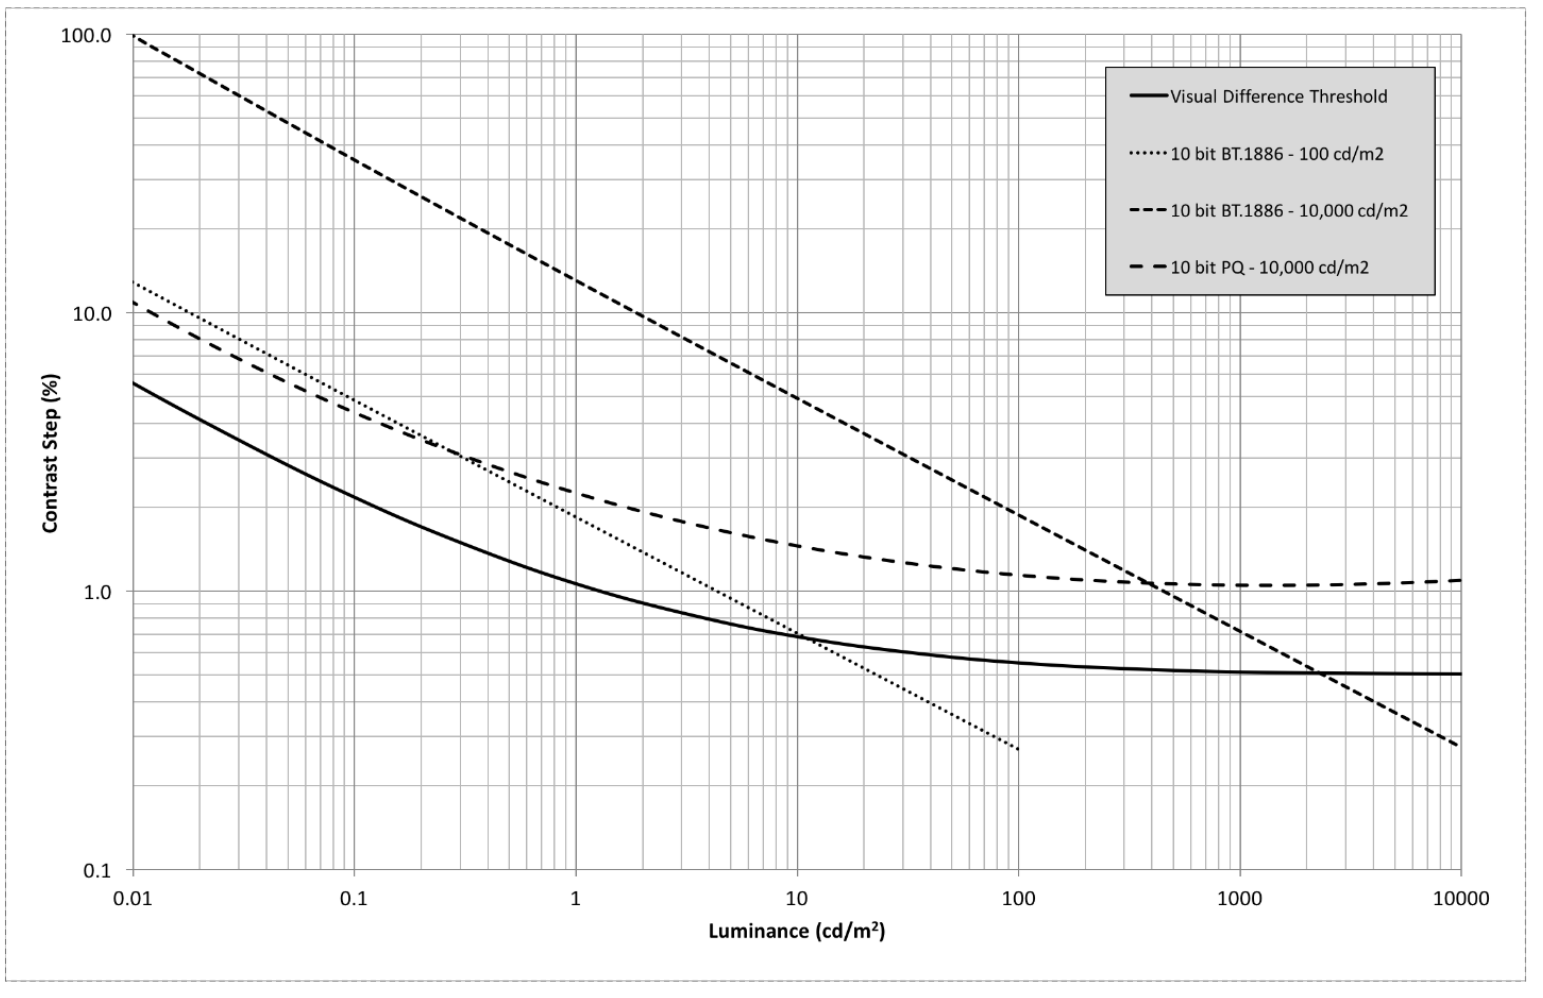
\includegraphics[width=12cm, keepaspectratio]{img/4_Formatos_de_TV_HDR/4_4_Agudeza_visual/1_barten_10bits.png}
  \caption{Relación entre el paso de contraste (\%) y la luminancia representable por un monitor (10 bits)}
  \label{fig:barten_10}
\end{figure}

Al contrario que el modelo de Barten, la \textcolor{green}{eotf} definida en \textit{ITU-R BT.1886} para los sistemas de televisión \textcolor{green}{hd}, y en general todas las funciones \textit{gamma} tradicionales, no es una aproximación precisa al \textcolor{green}{hvs}. Como resultado, 
\begin{figure}[H]
  \centering
  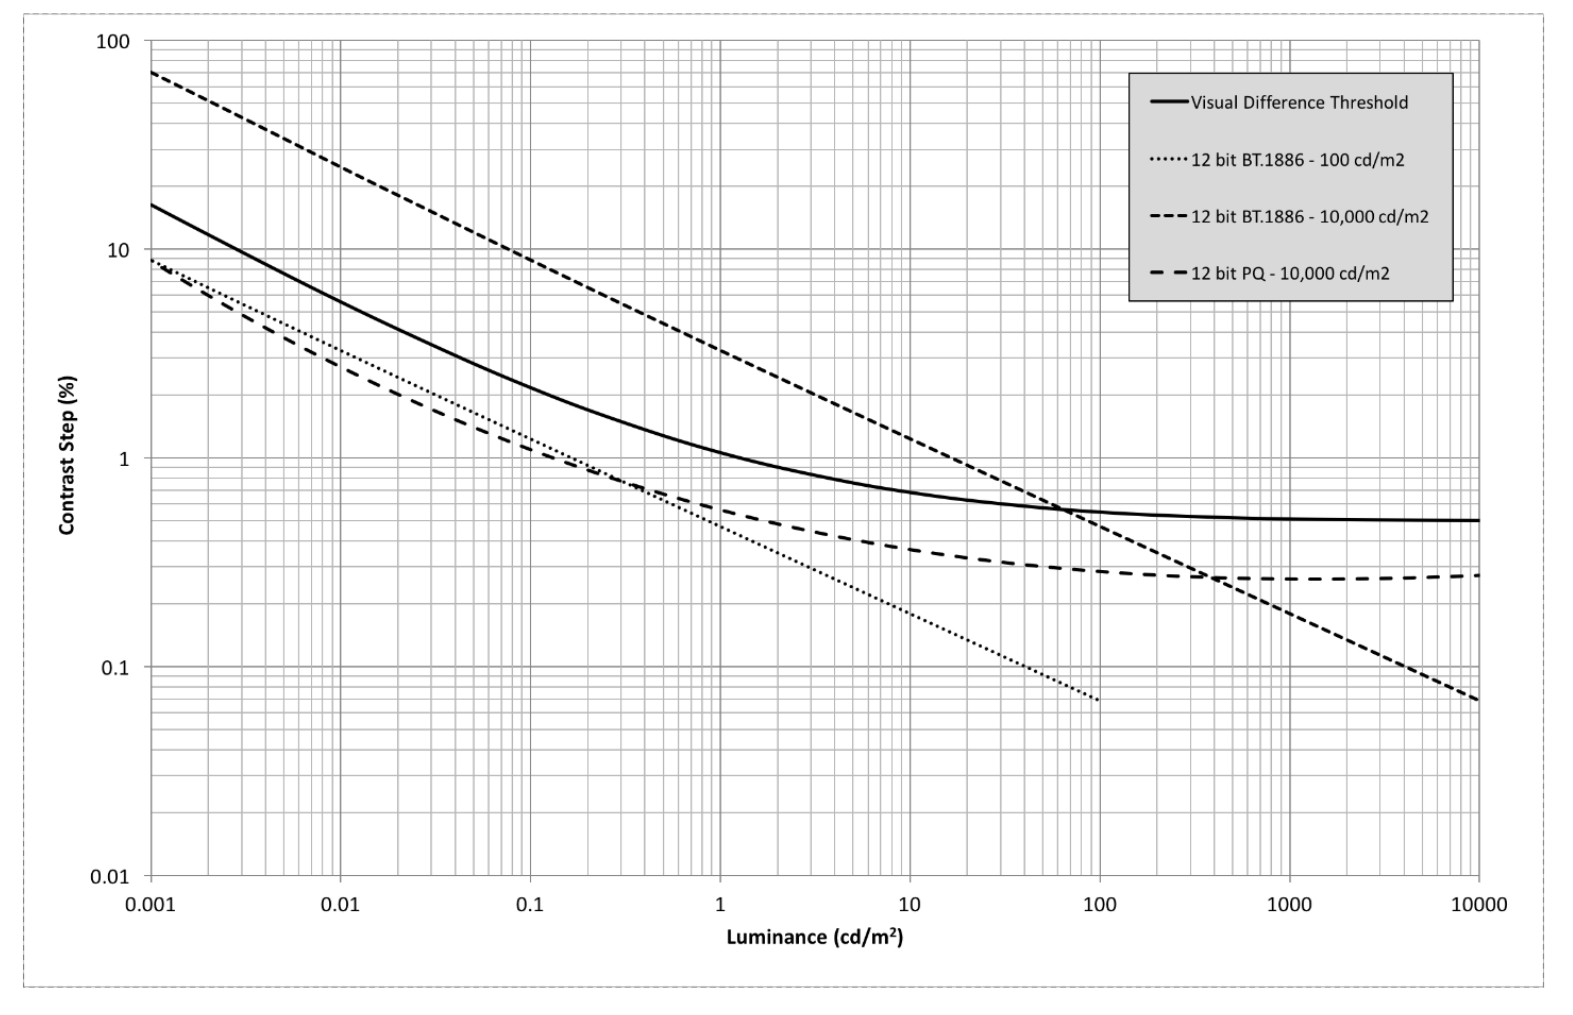
\includegraphics[width=12cm, keepaspectratio]{img/4_Formatos_de_TV_HDR/4_4_Agudeza_visual/2_barten_12bits.png}
  \caption{Relación entre el paso de contraste (\%) y la luminancia representable por un monitor (12 bits)}
  \label{fig:barten_12}
\end{figure}


\section{Condiciones de referencia}
\label{sec:condiciones_referencia}
    La  señal de vídeo \textcolor{green}{hdr} que es transmitida a través del sistema de distribución está calibrada y masterizada para ser visualizada en un monitor  de referencia, en un ambiente de referencia.
    
    Estas condiciones, de acuerdo con la normativa \textit{ ITU-R BT2100}, son las siguientes:

\begin{itemize}
  \item  El monitor en el que se presenta un  determinado contenido \textcolor{green}{hdr} debe ser capaz de producir unos niveles de luminancia mínimo y máximo de  $ 0.005 \nicefrac{cd}{m^{2}}$ y   $1000 \nicefrac{cd}{m^{2}}$ , respectivamente. 
  \item Entendiendo el entorno como el área que rodea al monitor (u otro dispositivo de visualización) y la periferia como el área restante de la superficie de visualización, los niveles de luminancia a los que deben mantenerse  dichas zonas es:
        \begin{itemize}
            \item Entorno:  $\:<5\: \nicefrac{cd}{m^{2}}$ 
            \item Periferia:  $\:5\: \nicefrac{cd}{m^{2}}$ 
        \end{itemize}
  \item  Tal y como se puede observar en la Tabla \ref{table:res_dis} distancia a la cual debe situarse un espectador para la observación crítica de contenidos HDR varía en función de la resolución de los contenidos presentados y de la naturaleza técnica de la evaluación de éstos.
\end{itemize}


\begin{table}[H]
\centering
\resizebox{\textwidth}{!}{%
\begin{tabular}{|c|c|l|c|c|}
\hline
\multirow{2}{*}{\textbf{Resolución}}                                         & \multicolumn{2}{c|}{\multirow{2}{*}{1920x1080 (1080p)}}                                            & \multirow{2}{*}{3840x2160 (2160p/4k)}                                            & \multirow{2}{*}{7860x4320 (4320p/8k)}                                        \\
                                                                             & \multicolumn{2}{c|}{}                                                                              &                                                                                  &                                                                              \\ \hline
\textbf{\begin{tabular}[c]{@{}c@{}}Distancia de \\ observación\end{tabular}} & \multicolumn{2}{c|}{\begin{tabular}[c]{@{}c@{}}3.2 veces la altura\\  de la pantalla\end{tabular}} & \begin{tabular}[c]{@{}c@{}}1.6-3.2 veces la\\ altura de la pantalla\end{tabular} & \begin{tabular}[c]{@{}c@{}}0.8 veces la altura\\ de la pantalla\end{tabular} \\ \hline
\end{tabular}%
}
\caption{Relación entre la resolución y la distancia de visualización}
\label{table:res_dis}
\end{table}
Los valores de la tabla de arriba fueron calculados teniendo en cuenta las siguientes consideraciones:

La agudeza visual del ojo humano ($\alpha$) es de aproximadamente  un minuto de arco, que equivale a 60 píxeles por grado. Tal y como se describe en la \textcolor{green}{itu} existe una distancia de visualización de imágenes digitales a partir de la cual el ojo humano no es capaz de distinguir dos píxeles adyacentes: la distancia de visualización óptima. Esta distancia es dependiente de las dimensiones y resolución de la pantalla de visualización y de la agudeza visual. Sin embargo, de acuerdo con la Ecuación \ref{eq:res_dis}, su valor es aproximadamente proporcional al cociente entre la altura de la pantalla y la resolución vertical de ésta, multiplicado por un factor constante.


\begin{equation} \label{eq:res_dis}
    \tan{\nicefrac{\alpha}{2}}= \frac{\nicefrac{(\nicefrac{H_{s}}{H_{r}})}{2}}{d} \qquad
    d_{opt}= \frac{\nicefrac{V_{s}}{V_{r}}}{2*tan(\nicefrac{1}{120})}\, \approx\,3438 \frac{V_{s}}{V_{r}}
\end{equation}
 
 Por ejemplo, dado un monitor de dimensiones $57x33cm$ y resolución $1920x1080$ (\textcolor{green}{hd}):
 La distancia óptima de observación es, aproximadamente $d_{opt}\, \approx \, 3438\frac{33}{1080}\, \approx \, 105 cm \, \approx \, 3.2 *33cm = 3.2 \: veces\: la\:  altura \: de \: la\:  pantalla\:$
 Estos resultados son coherentes con la Tabla \ref{table:res_dis}

\begin{figure}[H]
  \centering
  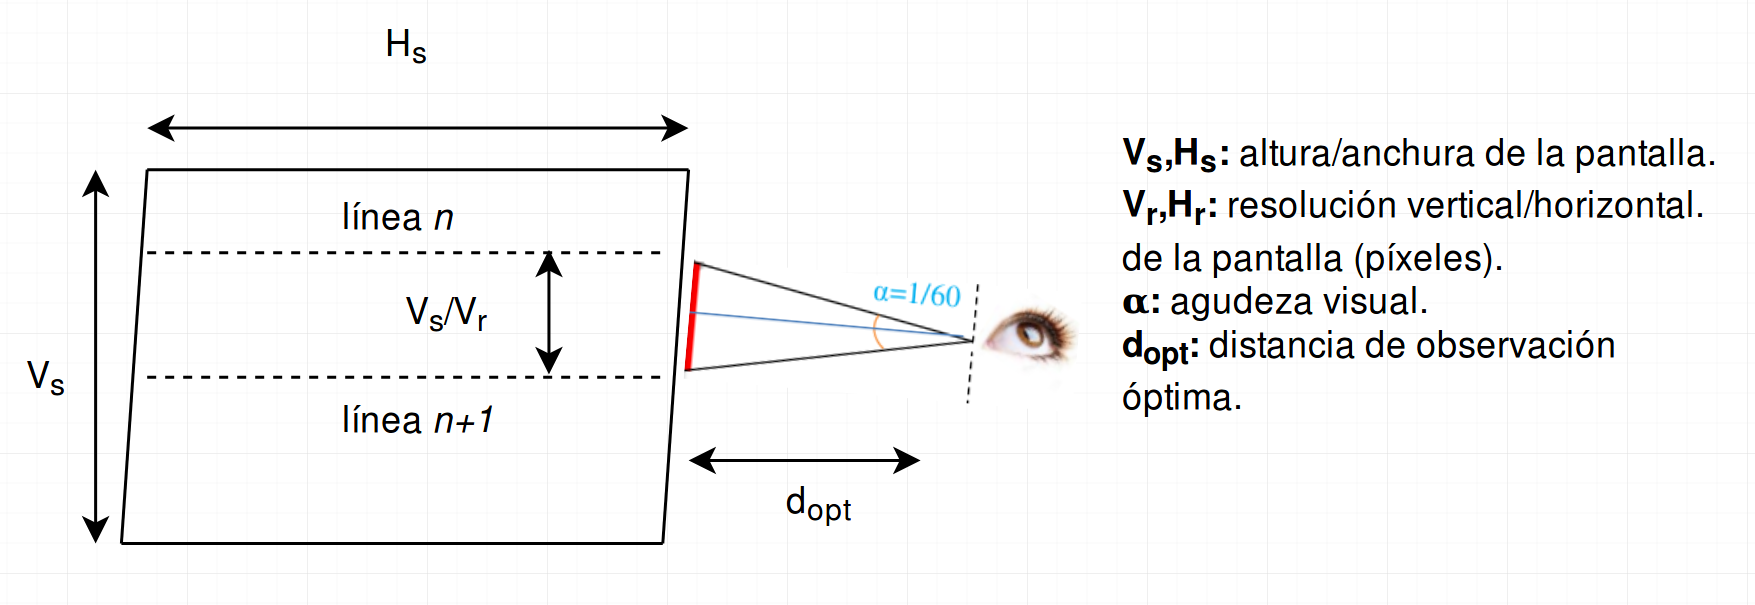
\includegraphics[width=10cm, keepaspectratio]{img/4_Formatos_de_TV_HDR/4_5_Condiciones_de_Referencia/1_resolution_vs_distance.png}
  \caption{Relación entre la agudeza visual y las dimensiones y resolución de la pantalla.}
  \label{fig:res_dist}
\end{figure}

\section{Conversiones entre formatos HDR}
\label{sec:conversiones_hdr}
Actualmente, para que un dispositivo de visualización pueda ser considerado HDR, debe soportar al menos el formato \textcolor{green}{hdr10}, el cual utiliza como funciones de transferencia las definidas en el sistema \textcolor{green}{pq}. Sin embargo, la incorporación de soporte \textcolor{green}{hlg} en dichos dispositivos no es obligatoria.

Por otro lado, los contenidos audiovisuales pueden haber sido producidos para ser renderizados  tanto en \textcolor{green}{pq} como en \textcolor{green}{hlg}. Por esta razón, a fin de  garantizar la capacidad de visualización de dichos contenidos en monitores sin soporte para el segundo de ellos, la  recomendación \textit{ITU-R BT.2390} propone diferentes mecanismos de conversión entre señales \textcolor{green}{hdr}.\\ En concreto, se definen tres métodos:

\begin{enumerate}
    \setlength\itemsep{-0.5em}
    \item Transcodificación de \textcolor{green}{pq} a \textcolor{green}{hlg}, el cual se desarrolla en la Subsección                     \ref{subsec:pq_a_hlg}.\label{item:pq_to_hlg}
    \item Transcodificación de \textcolor{green}{hlg} a \textcolor{green}{pq}, el cual se desarrolla en la Subsección                     \ref{subsec:hlg_a_pq}.\label{item:hlg_to_pq}
    \item Por último, la posibilidad de utilizar una \textcolor{green}{ootf} común a ambos formatos,
          descrito en la Subsección \ref{subsec:ootf_common}.\label{item:common_ootf}
\end{enumerate}


 

Tras la aplicación de los métodos (\ref{item:pq_to_hlg}) ó (\ref{item:hlg_to_pq}), se obtiene como resultado una señal que, tras su correspondiente decodificación, será reproducida por pantalla con el mismo nivel de luminancia pico que la señal original. No obstante, es condición necesaria que los monitores en los que se visualicen los contenidos posean el mismo nivel de luminancia pico.
 
Deben tenerse en cuenta las consideraciones anteriores y las diferencias existentes en la renderización de los formatos \textcolor{green}{pq} y \textcolor{green}{hlg} para su correcta representación en un monitor.
 
Mientras que el primero contempla la presentación de contenidos con un nivel de luminancia pico de hasta 10000 candelas por metro cuadrado, en el segundo se define la \textcolor{green}{eotf} mediante la  fijación  de  unos niveles de luminancia mínimo Lb y máximo Lw, escogidos  en función de las capacidades lumínicas de la pantalla objetivo. Por consenso de la industria audiovisual, con el objetivo de garantizar la consistencia de la conversión de formatos \textcolor{green}{hdr}, se fija en un nivel de luminancia pico común de  
1000 candelas por metro cuadrado.

\subsection{De PQ a HLG}
\label{subsec:pq_a_hlg}
Una vez se obtiene una señal \textcolor{green}{pq} limitada a $1000\: \nicefrac{cd}{m^{2}}$, la conversión de formato \textcolor{green}{pq} a \textcolor{green}{hlg} se lleva a cabo a través del diagrama de la Figura \ref{fig:pq_to_hlg_diag}.\\
Dada una señal \textcolor{green}{pq}, limitada a $1000\: \nicefrac{cd}{m^{2}}$:
\begin{itemize}
    \item Se aplica la \textcolor{green}{eotf} del sistema \textcolor{green}{pq} para obtener la señal óptica lineal pereparada para ser mostrada en un monitor \textcolor{green}{pq}.
    \item Se aplica la \textcolor{green}{inveotf} del sistema \textcolor{green}{hlg} para obtener la señal \textcolor{green}{hlg}.
    \item  Se aplica la \textcolor{green}{eotf} del sistema \textcolor{green}{hlg} para obtener las señales ópticas lineal pereparada para ser mostrada en un monitor \textcolor{green}{hlg}.
\end{itemize}

Respetando las limitaciones de la conversión anterior, la señal óptica (1) y (2) serán equivalentes.

\begin{figure}[H]
    \centering
    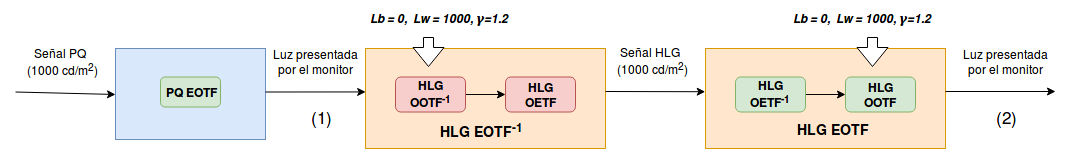
\includegraphics[width=16cm, keepaspectratio]{img/4_Formatos_de_TV_HDR/4_6_Conversiones_entre_Formatos_HDR/4_6_1_de_PQ_a_HLG/1_pq2hlg.png}
    \caption{Diagrama de conversión de formato PQ a HLG}    
    \label{fig:pq_to_hlg_diag}
\end{figure}
\subsection{De HLG a PQ}
\label{subsec:hlg_a_pq}

\begin{figure}[H]
    \centering
    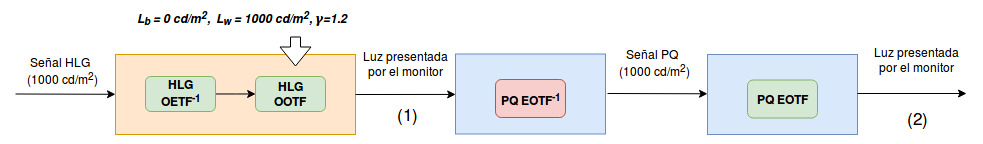
\includegraphics[width=16cm, keepaspectratio]{img/4_Formatos_de_TV_HDR/4_6_Conversiones_entre_Formatos_HDR/4_6_2_de_HLG_a_PQ/1_hlg2pq.png}
    \caption{Diagrama de conversión de formato HLG a PQ}
    \label{fig:hlg_to_pq_diag}
\end{figure}
\subsection{OOTF común}
\label{subsec:ootf_common}

Esta solución propone como alternativa utilizar una \textcolor{green}{ootf} de referencia común,la del sistema \textcolor{green}{pq} o la del sistema\textcolor{green}{hlg}; la cual puede ser modificada en la cámara para lograr el \textit{look} deseado.
Posteriormente las señales correspondientes serán decodificadas utilizando la \textcolor{green}{inveotf} correspondiente al formato deseado, ya sea \textcolor{green}{pq} o \textcolor{green}{hlg}.

La luz preparada para ser mostrada por pantalla, será igual en los puntos (1), (2.1) y (2.2), al igual que en los dos métodos anteriores.
Sin embargo, este sistema no requiere de la limitación inicial de la señal \textcolor{green}{pq} a $1000\: \nicefrac{cd}{m^{2}}$, ya que los contenidos son directamente grabados con dicha limitación.

\begin{figure}[H]
    \centering
    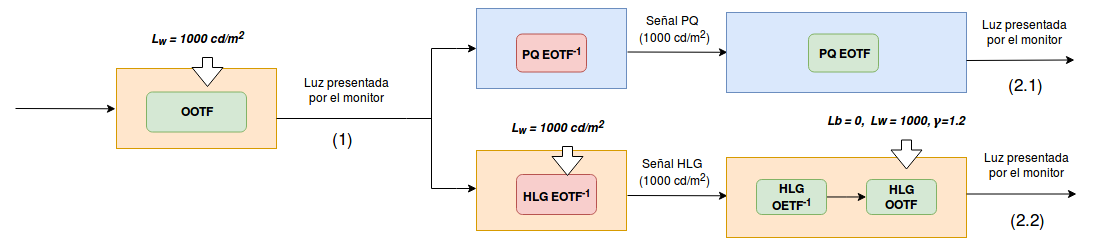
\includegraphics[width=16cm, keepaspectratio]{img/4_Formatos_de_TV_HDR/4_6_Conversiones_entre_Formatos_HDR/4_6_3_OOTF_comun/1_common_ootf.png}
    \caption{Diagrama del sistema OOTF común}
    \label{fig:ootf_common_diag}
\end{figure}

%%%%%%%%%%%%%%%%%%%%%%%%%%%%%%%%%%%%%%%%%%%%%%%%%%%%%%%%%%%%%%%%%%%%%%%%%%%%%%%%
%%%%%%%%%%%%%%%%%%%%%%%%%%%%%%%%%%%%%%%%%%%%%%%%%%%%%%%%%%%%%%%%%%%%%%%%%%%%%%%%
% TECNOLOGÍAS DE DESARROLLO DE LA APLICACIÓN %
%%%%%%%%%%%%%%%%%%%%%%%%%%%%%%%%%%%%%%%%%%%%%%%%%%%%%%%%%%%%%%%%%%%%%%%%%%%%%%%%

\cleardoublepage
\chapter{Tecnologías de desarrollo de la aplicación}
\textcolor{red}{No he añadido más información, pero... ¿es necesario hablar de Julia y R si no los voy a utilizar en el proyecto?}
\section{Jupyter (Notebook)}
\label{sec:Jupyter}

\textit{Jupyter Notebook\footnote{\url{https://jupyter.org/}}} es una herramienta web de código abierto que permite crear y compartir documentos con contenidos de naturaleza diversa. Está constituida por dos componentes:

\begin{itemize}
  \item  Una aplicación web, basada en el modelo cliente-servidor, que proporciona una interfaz gráfica
         para definir  y mostrar ecuaciones, texto explicativo, imágenes, etc. Además, permite la creación y ejecución de código en más de cuarenta lenguajes de programación, ofreciendo los resultados  correspondientes de ésta. Entre estos lenguajes destacan \textit{Python}, \textit{R} y \textit{Julia}, los cuales dan nombre al proyecto \textit{Jupyter}.
  \item Documentos de \textit{Jupyter Notebook} : son generados por el componente anterior y  contienen  información  sobre las entradas y salidas de  las operaciones computacionales, realizadas a través       de la interfaz. Tienen la extensión \textit{.ipynb}, un formato que es al mismo tiempo legible por humanos y ejecutable por la aplicación web. Estos documentos pueden ser  compartidos o visualizados a través de la herramienta de visualización de la comunidad \textit{Jupyter}: \textit{nbviewer\footnote{\url{http://nbviewer.jupyter.org/}}}, o exportados a \textit{LaTeX}, \textit{HTML}, \textit{PDF}, etc
\end{itemize}

\section{Python}
\label{sec:python}

\textit{Python\footnote{\url{https://www.python.org/}}} es un lenguaje de programación de propósito general, de alto nivel y orientado a objetos. Es  interpretado, es decir,  su código no necesita ser procesado por un compilador antes de ser ejecutado por la máquina.

Fue inventado por Guido van Rossum en 1989, basándose en los principios fundamentales del lenguaje informático \textit{ABC}, caracterizado por su simplicidad y facilidad de aprendizaje.

Entre sus características principales destacan:

\begin{itemize}
  \item La utilización de tipos de datos dinámicos, gracias a la cual es posible declarar tipos de datos mutables.
  \item La claridad de su sintaxis, que permite programar utilizando un menor número de líneas de código que en lenguajes como \textit{C++} y \textit{Java}.

  \item La portabilidad: existen intérpretes de python disponibles para gran cantidad de sistemas operativos.
  \item La sencillez en la  integración entre componentes de una aplicación, facilitando la comunicación entre 
        partes de una aplicación escritas en  \textit{Python} y otros lenguajes de programación como \textit{C}, \textit{C++}, \textit{Perl}, \textit{Java}, etc.
\end{itemize}

Además, proporciona una vasta librería  estándar que incluye funcionalidades para  diferentes áreas, tales como el procesado de cadenas de caracteres, la gestión de protocolos de internet y la ingeniería de software.

%%%%%%%%%%%%%%%%%%%%%%%%%%%%%%%%%%%%%%%%%%%%%%%%%%%%%%%%%%%%%%%%%%%%%%%%%%%%%%%%
%%%%%%%%%%%%%%%%%%%%%%%%%%%%%%%%%%%%%%%%%%%%%%%%%%%%%%%%%%%%%%%%%%%%%%%%%%%%%%%%
% DISEÑO E IMPLEMENTACIÓN %
%%%%%%%%%%%%%%%%%%%%%%%%%%%%%%%%%%%%%%%%%%%%%%%%%%%%%%%%%%%%%%%%%%%%%%%%%%%%%%%%
\cleardoublepage
\chapter{Diseño e implementación}


\section{Arquitectura general} 
\label{sec:arquitectura}

\section{Sistema PQ} 
\label{sec:sistema_pq_tool}

\section{Sistema HLG} 
\label{sec:sistema_hlg_tool}

\section{Conversiones entre formatos HDR} 
\label{sec:conversiones_formatos_hdr}



%%%%%%%%%%%%%%%%%%%%%%%%%%%%%%%%%%%%%%%%%%%%%%%%%%%%%%%%%%%%%%%%%%%%%%%%%%%%%%%%
%%%%%%%%%%%%%%%%%%%%%%%%%%%%%%%%%%%%%%%%%%%%%%%%%%%%%%%%%%%%%%%%%%%%%%%%%%%%%%%%
% SECUENCIAS DE TEST PARA ENSAYOS %
%%%%%%%%%%%%%%%%%%%%%%%%%%%%%%%%%%%%%%%%%%%%%%%%%%%%%%%%%%%%%%%%%%%%%%%%%%%%%%%%

\cleardoublepage
\chapter{Secuencias de test para ensayos}


%%%%%%%%%%%%%%%%%%%%%%%%%%%%%%%%%%%%%%%%%%%%%%%%%%%%%%%%%%%%%%%%%%%%%%%%%%%%%%%%
%%%%%%%%%%%%%%%%%%%%%%%%%%%%%%%%%%%%%%%%%%%%%%%%%%%%%%%%%%%%%%%%%%%%%%%%%%%%%%%%
% CONCLUSIONES %
%%%%%%%%%%%%%%%%%%%%%%%%%%%%%%%%%%%%%%%%%%%%%%%%%%%%%%%%%%%%%%%%%%%%%%%%%%%%%%%%

\cleardoublepage
\chapter{Conclusiones}
\label{chap:conclusiones}

\section{Consecución de objetivos}
\label{sec:consecucion-objetivos}

\section{Aplicación del conocimiento}
\label{sec:aplicacion}
En el transcurso de mi grado, Ingeniería en Sistemas Audiovisuales y Multimedia (ISAM), he adquirido diversos conocimientos y  aprendido a manejar diferentes herramientas que me han facilitado el desarrollo de este proyecto. Entre las principales asignaturas que engloban dicho aprendizaje, destacan:
\begin{enumerate}
  \item \textbf{`` Informática I ''}: Con esta materia comenzó mi inmersión en el área de la programación algorítmica. En ella aprendí conceptos básicos como el uso de datos tipados y  el manejo de estructuras de control.
  
  \item \textbf{`` Protocolos para la Transmisión de Audio y Vídeo ''}: Al cursar esta materia, adquirí conocimientos en programación orientada a objetos, a través de diversas prácticas desarrolladas en el lenguaje informático interpretado \textit{Python}.
  
  \item \textbf{`` Tratamiento Digital de la Imagen ''}: Esta materia me introdujo en el campo del análisis de imagen digital, aprendiendo diferentes técnicas de procesado (segmentación y morfología), filtrado (espacial y frecuencial) y transformación entre espacios de color ( afianzado en asignaturas como Difusión de Audio y Vídeo y Equipos y Sistemas de Audio y Vídeo).
  
  \item \textbf{`` Estándares de Codificación de Audio y Vídeo ''}: Gracias a está materia fui capaz de comprender las limitaciones de los sistemas auditivo y visual humanos, así como su influencia en el diseño eficiente de códecs de audio y vídeo.
  
  \item \textbf{`` Equipos y Sistemas de Audio y Vídeo ''}: Esta asignatura es la razón por la cual comencé el desarrollo de este proyecto. En ella, fui introducido a la tecnología HDR (High Dynamic Range), que permite visualización / presentación  de contenidos audiovisuales en una pantalla, preservando las características con las que fueron masterizadas.  

 Por otro lado, adquirí una visión general de la estructura de un centro de producción audiovisual, la diversidad de formatos utilizados en éste y las interfaces de transporte de contenidos (SD-SDI, HD-SDI) empleadas. Gracias a ello, he podido entender las diferentes transformaciones que sufre una señal de vídeo tras su paso por la cadena completa, así como las posibles degradaciones derivadas de ellas.
 
 \textbf{\textit{Posiblemente incluya: Sistemas Lineales y Álgebra}}
\end{enumerate}


\section{Lecciones aprendidas}
\label{sec:lecciones_aprendidas}

\section{Trabajos futuros}
\label{sec:trabajos_futuros}


%%%%%%%%%%%%%%%%%%%%%%%%%%%%%%%%%%%%%%%%%%%%%%%%%%%%%%%%%%%%%%%%%%%%%%%%%%%%%%%%
%%%%%%%%%%%%%%%%%%%%%%%%%%%%%%%%%%%%%%%%%%%%%%%%%%%%%%%%%%%%%%%%%%%%%%%%%%%%%%%%
% APÉNDICE(S) %
%%%%%%%%%%%%%%%%%%%%%%%%%%%%%%%%%%%%%%%%%%%%%%%%%%%%%%%%%%%%%%%%%%%%%%%%%%%%%%%%

\cleardoublepage
\appendix

\chapter{Desarrollo}
\section{Método de derivación de las coordenadas de los valores tristímulus \textit{XYZ} a partir de las componentes \textit{RGB}}
\label{sec:rgb_to_xyz}

 \begin{enumerate}
     \item  En primer lugar, partiendo de las coordenadas \textit{xy} del blanco de referencia \textit{D65} y las \textit{chromaticities} definidas por un determinado espacio de color, la componente \textit{z} es derivada:
         \begin{equation}
             z = 1 - (x + y)
         \end{equation}
     \item Composición de las matrices \textit{P} y \textit{W}, correspondientes a las \textit{chromaticities} de cada una de las componentes primarias \textcolor{green}{rgb} y el blanco de referencia, respectivamente:
        \begin{equation}
            P = \begin{bmatrix}
                    x_R & x_G & x_B \\
                    y_R & y_G & y_B \\
                    z_R & z_G & z_B
                \end{bmatrix}
            \hspace{2cm}
            W = \begin{bmatrix}
                    \nicefrac{x_W}{y_W}\\
                    1 \\
                    \nicefrac{z_W}{y_W}
            \end{bmatrix}
        \end{equation}
    \item Cálculo de los coeficientes $C_i$:
        \begin{equation}
            \begin{bmatrix}
                C_R\\
                C_G\\
                C_B
            \end{bmatrix} = P^{-1}\cdot W
            \hspace{0.5cm}\Longrightarrow\hspace{0.5cm}
            C = \begin{bmatrix}
                    C_R & 0 & 0 \\
                    0 & C_G & 0 \\
                    0 & 0 & C_B
                \end{bmatrix}
        \end{equation}
    \item Cálculo de la matriz de normalización primaria (NPM) como el producto matricial de las coordenadas de las tres componentes primarias por sus respectivos coeficientes:
        \begin{equation}
             NPM = P\cdot C = \begin{bmatrix}
                                X_R & X_G & X_B \\
                                Y_R & Y_G & Y_B \\
                                Z_R & Z_G & Z_B
                             \end{bmatrix}
        \end{equation}
    \item Obtención de la matriz de conversión de \textcolor{green}{rgb} a \textcolor{green}{xyz}:
        \begin{equation}
             \begin{bmatrix}
                X\\
                Y\\
                Z
            \end{bmatrix}  =
            \underbrace{\begin{bmatrix}
                X_R & X_G & X_B \\
                Y_R & Y_G & Y_B \\
                Z_R & Z_G & Z_B
            \end{bmatrix}}_{NPM} \cdot 
            \begin{bmatrix}
                R\\
                G\\
                B
            \end{bmatrix}
            \textrm{ donde   }
            Y = Y_R \cdot R + Y_G \cdot G + Y_B \cdot B
        \end{equation}
        
 \end{enumerate}
 
 
 Para obtener la matriz de conversión de \textcolor{green}{xyz} a \textcolor{green}{rgb} se calcula la inversa de la matriz \textit{NPM} correspondiente:
    \begin{equation}
        \begin{bmatrix}
            R\\
            G\\
            B
        \end{bmatrix}  =
        \underbrace{\begin{bmatrix}
            X_R & X_G & X_B \\
            Y_R & Y_G & Y_B \\
            Z_R & Z_G & Z_B
        \end{bmatrix}^{-1}}_{NPM^{-1}} \cdot 
        \begin{bmatrix}
            X\\
            Y\\
            Z
        \end{bmatrix}
    \end{equation}
    
\section{Conversión entre diferentes sets de coordenadas RGB}
\label{sec:rgbs_to_rgbd}
    Este método establece las directrices a seguir para realizar la conversión de un detrminado \textit{set} de coordenadas primarias aditivas (\textcolor{green}{rgb}) a otro. Este proceso es también válido para la transformación de coordenadas \textcolor{green}{rgb} de referencia a las presentadas en un \textit{display}.
    
    Teniendo en cuenta que los subíndices $_S$ y $_D$ hacen referencia a las señales origen y destino, respectivamente:
        \begin{equation}
        \begin{bmatrix}
                R_S\\
                G_S\\
                B_S
         \end{bmatrix} =
         NPM^{-1}_S\cdot
         \begin{bmatrix}
            X\\
            Y\\
            Z
        \end{bmatrix},  
        \begin{bmatrix}
            R_D\\
            G_D\\
            B_D
        \end{bmatrix} =
         NPM^{-1}_D\cdot
         \begin{bmatrix}
            X\\
            Y\\
            Z
        \end{bmatrix}
    \end{equation}
    
    Los valores \textcolor{green}{xyz}, al ser dependientes de las características del ojo humano, deben ser iguales tanto en las matrices origen como destino(\textcolor{red}{¿Por qué?}). Por tanto, se puede derivar la siguiente ecuación:
    
    \begin{equation}
          \begin{bmatrix}
            R_D\\
            G_D\\
            B_D
          \end{bmatrix} =
          \underbrace{NPM_D^{-1} \cdot NPM_S}_{TRA} \cdot
          \begin{bmatrix}
            R_S\\
            G_S\\
            B_S
          \end{bmatrix},
    \end{equation}
    donde \textit{TRA} es la matriz de conversión que satisface dicha transformación.
\chapter{Definiciones}
\label{app:definiciones}

\section{Magnitudes físicas relacionadas con la luz}
\label{sec:fisica_luz}

\begin{itemize}
    \item \textbf{Espectro óptico: } es el rango de longitudes de onda dentro del espectro electromagnético que engloba a la luz ultravioleta, visible e infrarroja ({\footnotesize $10-10^{6} nm$}). El intervalo comprendido entre {\footnotesize $330 nm$} y {\footnotesize $780 nm$} se corresponde con el espectro visible, tal y como se muestra en la Figura \ref{fig:visible_spectrum}.

\begin{figure}[H]
    \centering
    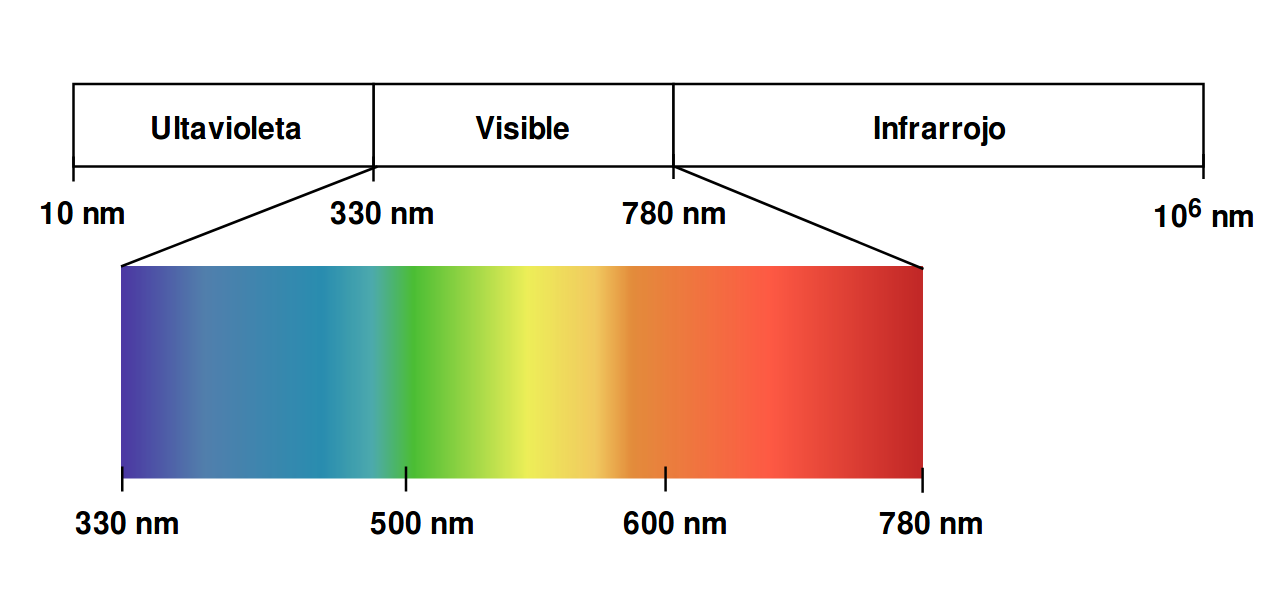
\includegraphics[width=11cm, keepaspectratio]{img/APENDICES/B/optic_spectrum.png}
    \caption{Espectro óptico}
    \label{fig:visible_spectrum}
\end{figure}
    
    \item \textbf{Flujo radiante {\footnotesize ($\phi$)}:} en el rango de longitudes de onda del espectro óptico, es la cantidad de energía que una fuente es capaz de radiar sobre una superficie por unidad de tiempo. Se designa como y su unidad es el \textit{watio (w)}.
    
    \item \textbf{Flujo luminoso {\footnotesize ($\phi_{v}$}):} en el espectro visible, es la porción de energía luminosa que es irradiada sobre una superficie por unidad de tiempo. Esta magnitud es obtenida como un subconjunto ponderado y promediado del flujo radiante, que se basa en la sensibilidad variable del ojo humano a la intensidad luminosa en función de {\footnotesize $\lambda$}. Su unidad de medida es el \textit{lumen}.
    
    \item \textbf{Candela: } se define como la sexagésima parte de la instensidad luminosa emitida por un cuerpo negro radiante de {\footnotesize $ 1\:cm^2$} a 2042º K, la temperatura de fusión del platino sólido. También puede interpretarse como la intensidad luminosa que una fuente de radiación monocromática es capaz de emitir en una dirección determinada a una longitud de onda de {\footnotesize $555 \, nm$}. Tal y como se puede observar en la Figura \ref{fig:func_luminosidad}, para dicho valor de {\footnotesize $\lambda$}, la respuesta del ojo humano a la luminosidad es máxima: {\footnotesize $683\, \nicefrac{lumens}{w}$}.
    
    \begin{figure}[H]
        \centering
        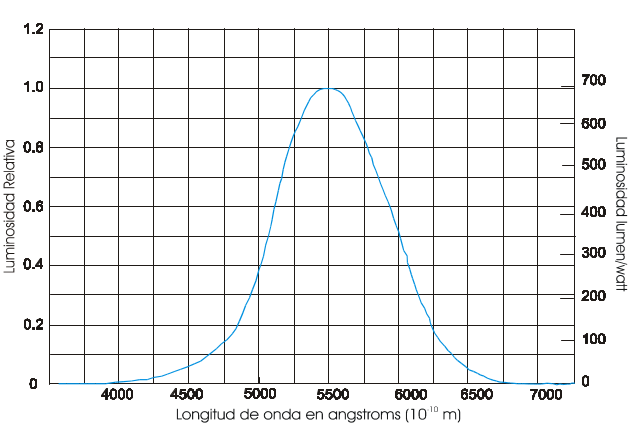
\includegraphics[width=10cm, keepaspectratio]{img/APENDICES/B/tf_luminosidad.png}
        \caption{Respuesta del ojo humano a la luz monocromática (función de luminosidad)}
        \label{fig:func_luminosidad}
    \end{figure}
    \item \textbf{Lumen:} es la unidad de medida del \textit{flujo luminoso} emitido por una fuente con una intensidad uniforme de una candela por unidad de ángulo sólido; o bien el \textit{flujo luminoso} irradiado sobre una unidad de área que cumple que todos sus puntos se encuentran a distancia unidad de la fuente.
    
\end{itemize}


\section{Unidades de medida de luminancia}
\label{sec:luminance_units}

La luminancia se define como la porción de energía luminosa  del espectro visible que una determinada superficie es capaz de emitir o reflejar. Este parámetro puede ser medido en diversas unidades:

    
    %\item \textbf{Stilb {\footnotesize ($\nicefrac{cd}{cm^{2}}$)}} : {\footnotesize equivale a $10^{4}\: \nicefrac{cd}{m^{2}}$}.
    
    %\item \textbf{Lambert} {\footnotesize ($\nicefrac{lumen}{cm^{2}}$)}:  equivale a {\footnotesize{$\frac{10^{4}}{\pi} \, \nicefrac{cd}{m^{2}}$}}.
    
    %\item \textbf{Foot Lambert} {\footnotesize ($ftL = \nicefrac{lumen}{pie^{2}}$)}:
\begin{enumerate}
    \item \textbf{Candela por metro cuadrado {\footnotesize ($\nicefrac{cd}{m^{2}}$)}}: también conocida informalmente como \textit{nit}, es la unidad utilizada por el \textcolor{green}{si}.
    
    \item \textbf{Candela por pie cuadrado {\footnotesize ($\nicefrac{cd}{pie^{2}}$)}} : es la unidad utilizada por el     sistema inglés, que equivale a {\footnotesize $10.76\: \nicefrac{cd}{m^{2}}$}.

    
    \item \textbf{Lux} {\footnotesize ($\nicefrac{lumen}{m^{2}}$)}: utilizada para cuantificar la luz incidente sobre una superficie.
    
\end{enumerate}

\textcolor{red}{Mis fuentes han sido ~\cite{url:_vision_luz_color}}
%\begin{itemize}%
    %\item \url{http://personales.unican.es/perezvr/pdf/Vision%20Luz%20y%20Color.pdf}
    %\item \url{https://recursos.citcea.upc.edu/llum/fotometria/magnitud.html}
    %\item \url{http://hyperphysics.phy-astr.gsu.edu/hbasees/vision/lumpow.html}
    %\item \url{https://www.bipm.org/en/publications/si-brochure/candela.html}
%\end{itemize}%


\chapter{Manual de usuario}
\label{app:manual}
%%%%%%%%%%%%%%%%%%%%%%%%%%%%%%%%%%%%%%%%%%%%%%%%%%%%%%%%%%%%%%%%%%%%%%%%%%%%%%%%
%%%%%%%%%%%%%%%%%%%%%%%%%%%%%%%%%%%%%%%%%%%%%%%%%%%%%%%%%%%%%%%%%%%%%%%%%%%%%%%%
% BIBLIOGRAFIA %
%%%%%%%%%%%%%%%%%%%%%%%%%%%%%%%%%%%%%%%%%%%%%%%%%%%%%%%%%%%%%%%%%%%%%%%%%%%%%%%%

\cleardoublepage

% Las siguientes dos instrucciones es todo lo que necesitas
% para incluir las citas en la memoria
\bibliographystyle{unsrt}
\bibliography{memoria}  % memoria.bib es el nombre del fichero que contiene
% las referencias bibliográficas. Abre ese fichero y mira el formato que tiene,
% que se conoce como BibTeX. Hay muchos sitios que exportan referencias en
% formato BibTeX. Prueba a buscar en http://scholar.google.com por referencias
% y verás que lo puedes hacer de manera sencilla.
% Más información: 
% http://texblog.org/2014/04/22/using-google-scholar-to-download-bibtex-citations/

%\textcolor{green}{itu}
%\textcolor{green}{itur}
%\textcolor{green}{smpte}
%\textcolor{green}{d65}
\end{document}
